\chapter{Appendix of ``Endogenous taxation in ongoing internal conflict: The case of Colombia'' \label{chap:append3}}

%%----------------------------------------%%
\section{Data \label{data_appendix3}}

\subsection{Tax Revenue and Institutions \label{appendix3:taxrevenues&institutions}}

Our data on local tax revenue come from the National Planning Department (Departamento Nacional de Planeaci\'{o}n (DNP)), which compiles the data from the municipalities. Municipal authorities submit a quarterly form called the ``Unique Tributary Form'' (Formato \'Unico Tributario (FUT)), which is sent to the Ministry of Finance. The DNP processes the information as annual averages with a roughly 4-year lag. As noted above, the primary source of local tax revenue is the property tax. We estimate the logged average of local tax revenues at the municipal level for each of the time periods that characterize the Colombian civil war since the 1980s (subsection on ``Civil War and Capture in Colombia''). 

To measure other aspects of tax institutions, we constructed four variables using publicly available data from IGAC, the national land registry service: the per capita land value, the number of land registry updates, the time elapsed since the last registry update, and the land informality rate per municipality. 

\subsection{Violence \label{appendix3:violence}}

Our main explanatory variables are violence by guerillas and paramilitary groups at the municipal level. As noted in $H_1a$ above, we expect that violence perpetrated by the FARC is likely to have a  negative impact on tax collection and formality. In contrast, as noted in $H_2a$, paramilitary activity is expected to be associated with formalization in favor of their landholding supporters and therefore greater net tax receipts.

Our data on violence at the municipal level was compiled by \citet{restrepoetal03}, and updated by Universidad el Rosario through 2014. The data record for every event its location and date, its perpetrator and type (distinguishing between unilateral bellicose activities like guerrilla attacks, and combats between two of the conflict parties), and the resulting casualties. To assess net influence in a given time period, we aggregated all attacks by armed groups of a certain type over the periods described in the subsection on ``Civil War and Capture in Colombia'', normalize for population, and log the resulting cumulative variable given the existent skewness. Note that this monotonic transformation effectively reduces the weights of outliers in the specification as a way for correcting for such.

\subsection{Electoral outcomes \label{appendix3:electoral_outcomes}}

Electoral data on all local elections from 1997 to 2011 was compiled by \citet{pachonsanchez14}, suing as a primary source the reports of {\it Registradur\'ia Nacional del Estado Civil}, Colombia's electoral and identity bureau. Both mayor and city councils were elected in 1997, 2000, 2003, 2007 and 2011. Elected officials had three-year terms until 2003, when terms extended to four years.

Because right wing parties had clear tax policy preferences we measure political alignment with a dummy variable equal to 1 if the elected mayor belong to the President's Uribe 2000s political party coalition, 0 otherwise. The coalition included the Conservative Colombian party and the following right- or center-right-wing parties: Cambio Radical, Partido Social de Unidad Nacional (Partido de la U), Colombia Democr\'atica, Convegencia Ciudadana and Alas Equipo Colombia.

\subsection{Social outcomes and economic activity \label{appendix3:social_outcomes}}

Municipal governments in Colombia provide a series of social outcomes through public good services, and thus are subject to potential effects by armed groups, through a capture of local authorities (see Appendix \label{appendix3:test_electoral_mechanism}). 

We rely on social outcomes from DANE such as secondary enrollment and measures of quality of education through math scores of standardized national tests (SABER 11).  

Lastly, to measure economic activity at the municipal level over the period from 1997 to 2013, we rely on nighttime light data. Specifically, we use version 4 of the data collected by the Defense Meteorological Satellite Program (DMSP-OLS), and available through the National Oceanic and Atmospheric Administration's (NOAA) National Center for Environmental Information (NECI).\footnote{The DMSP satellites take images with a resolution of 30 arc-seconds (roughly 1 square km at the equator). The imagery removes snow, clouds, fires, gas flares and other ephemeral lights. Each 30 arc-second pixel has a 0 to 63 digital number assigned according to its luminosity intensity. However, due to problems related to degradation of the sensors, satellites trajectory and scanning procedure, and the differences in crossing time between satellites, the data suffers from a series of problems that affects it comparability across time. These include: discrepancies in the digital number among satellites from the same year; abrupt abnormal fluctuations in digital number values for different years, for the same satellite; substantial differences in the number of lit pixels for satellite at the same year; geographic misalignment; and, most importantly, blurring due to light over glow across space, which increases as the digital number grows, and thus biases more luminous areas (Baugh et al. 2010; Elvidge et al, 2009; Liu et al, 2012; Zhang \& Seto, 2011). Thus, to assure comparability across time and between satellites we intercalibrated the data following Wu et al. (2013), perform a geometric correction following  Zhao et al. (2015), and estimate an intra-annual composition for the cases where two satellites captured light for the same time period. Pixels who appeared in one of the satellites but not the other where labeled as unstable lit pixels and turned into missing values. The remaining stable lit pixels' digital numbers where averaged, a process which produced one intra-annual composite by year.}   Luminosity data recorded by satellites have been shown to be a consistent predictor of economic activity at both national and sub-national levels \citep{vernon11, bleakley2012, michalopoulos2013, storeygard2012, pinkosalai2014}, and have even been used for border-specific economic performance comparisons across very short geographical spaces \citep{pinko2013}. Recent work using geo-located Demographic and Health Survey (DHS) data confirm that luminosity tracks well with sub-national measures of economic activity in a range of developing world settings \citep{weidmann2017}.

\subsection{Other variables \label{appendix3:other_vars}}

Our dataset also contains a number of important controls including other fiscal measures  (such as transfers from the central government and royalties from the exploitation of natural resources), geographical characteristics of municipalities related to state presence and economic isolation such as the distance to the department's capital, pre-period vote share by political party ideology which is particularly important when measuring the effect of presence of armed groups on electoral outcomes, a dummy variable on whether a municipality had no registered homicides in the same period as the cumulative attack variable (to avoid a selection bias on armed group presence), the number of military bases in each time period from 1999 to 2009 to account for extra-normal state presence, and the number of people displaced, driven out, and received  by municipality due to conflict, which is important when assessing electoral outcomes. We also include an additive endowment index on the municipality production of gold, silver, platinum, nickel, emeralds and iron. Coca production levels are also included given the rapacity effect that this illegal market may generate on both armed groups' behavior.  

Table \ref{appendix3:descriptive} reports the descriptive statistics of all the variables (except the main variables, described in Table \ref{chapter3_tab:descriptive}). In turn, Table \ref{appendix3:description_vars} provides further details on the variables' sources.

%%-----------------------------------------------------------%
%Table 1A

\begin{table}[h]\centering \caption{Descriptive statistics of additional variables}
\label{appendix3:descriptive}
\scalebox{0.6}{
\begin{tabular}{l c c c c c}\hline\hline
\multicolumn{1}{c}{\textbf{Variable}} & \textbf{Mean}
 & \textbf{Std. Dev.}& \textbf{Min.} &  \textbf{Max.} & \textbf{N}\\ \hline
 \\
\multicolumn{6}{c}{Panel A. Outcomes }\\ 
 
{\it Social outcomes}	&		&		&		&		&		\\ 

Secondary enrollment rate 2003-2006&        0.60&        0.22&           0&           2&        1128\\
Quality of education (average math score) 2003-2006&       -0.16&        0.16&          -1&           1&         972\\



\\
{\it Economic activity}	&		&		&		&		&		\\ 

Log luminosity per capita 1997-2002&       -8.42&        1.11&         -12&          -4&        1063\\
Log luminosity per capita 2003-2006&       -8.52&        1.10&         -12&          -4&        1063\\
Log luminosity per capita 2007-2010&       -8.27&        1.15&         -12&          -4&        1063\\
Log luminosity per capita 2011-2013&       -8.33&        1.18&         -13&          -4&        1063\\


\\
{\it Vote share by political party coalition (Mayor elections)
}	&		&		&		&		&		\\ 

Uribe + Conservative party coalition 1997 and 2000 Mayor elections&        0.26&        0.32&           0&           1&        1020\\
Uribe + Conservative party coalition 2003 Mayor election&        0.22&        0.26&           0&           1&         914\\
Uribe + Conservative party coalition 2007 Mayor election&        0.58&        0.31&           0&           1&        1112\\
Uribe + Conservative party coalition 2003 and 2007 Mayor elections&        0.43&        0.26&           0&           1&        1114\\
Uribe + Conservative party coalition 2011 Mayor election&        0.41&        0.33&           0&           1&        1046\\



\\
{\it Vote share by political party coalition (City Council elections)
}	&		&		&		&		&		\\ 

Uribe + Conservative party coalition 1997 and 2000 City Council elections&        0.28&        0.24&           0&           1&        1101\\
Uribe + Conservative party coalition 2003 and 2007 City Council elections&        0.42&        0.18&           0&           1&        1114\\
Uribe + Conservative party coalition 2011 City Council election&        0.37&        0.20&           0&           1&        1046\\


\\
\multicolumn{6}{c}{Panel B. Violence}\\
{\it Violence (no-logs; with Table \ref{chapter3_tab:main} third period specification sample)}	&		&		&		&		&		\\ 

Guerrilla attacks per 100,000 inh. 1988-1996&       62.67&      118.76&           0&        1260&        1182\\
Paramilitary attacks per 100,000 inh. 1988-1996&       36.31&       74.22&           0&        1742&        1182\\
Guerrilla attacks per 100,000 inh. 1997-2002&       76.32&      128.62&           0&        1734&        1182\\
Paramilitary attacks per 100,000 inh. 1997-2002&       38.08&       56.12&           0&         581&        1182\\
Guerrilla attacks per 100,000 inh. 2003-2006&      116.18&      283.43&           0&        3372&        1182\\
Paramilitary attacks per 100,000 inh. 2003-2006&       30.01&       59.28&           0&         672&        1182\\
Guerrilla attacks per 100,000 inh. 2007-2010&       73.51&      169.31&           0&        1873&        1182\\
Paramilitary attacks per 100,000 inh. 2007-2010&       32.31&       60.71&           0&         672&        1182\\



\\

{\it Violence distribution moments (to compute marginal effects)} & \textbf{Median} & \textbf{p(90)}&  &   & \\
 Guerrilla attacks per 100,000 inh. 1988-1996&       17.44&      185.90\\
Paramilitary attacks per 100,000 inh. 1988-1996&       20.44&       94.55\\
Guerrilla attacks per 100,000 inh. 1997-2002&       35.83&      211.92\\
Paramilitary attacks per 100,000 inh. 1997-2002&       22.50&      102.23\\
Guerrilla attacks per 100,000 inh. 2003-2006&       24.57&      308.50\\
Paramilitary attacks per 100,000 inh. 2003-2006&       12.30&       83.92\\
Guerrilla attacks per 100,000 inh. 2007-2010&       16.81&      210.98\\
Paramilitary attacks per 100,000 inh. 2007-2010&       14.04&       89.45\\

 
  Guerrilla attacks per 100,000 inh. 2003-2010 \footnote{Using Table 6, panel A, third period specification sample.}&       53.16&      461.66\\
Paramilitary attacks per 100,000 inh. 2003-2010 \footnote{\emph{Same as last footnote.}}&       14.35&       89.49\\



\\

\multicolumn{6}{c}{Panel C. Controls}\\
{\it Vote share by political party ideology (Mayor elections)
}	&		&		&		&		&		\\ 

Left-wing party 1994&        0.02&        0.13&           0&           1&        1182\\
Traditional party 1994&        0.73&        0.44&           0&           1&        1182\\
Third (right-wing) party 1994&        0.24&        0.43&           0&           1&        1182\\
Indigenous Afro-Colombian party 1994&        0.01&        0.09&           0&           1&        1182\\
Left-wing party 2000&        0.01&        0.08&           0&           1&        1182\\
Traditional party 2000&        0.51&        0.50&           0&           1&        1182\\
Third (right-wing) party 2000&        0.47&        0.50&           0&           1&        1182\\
Indegenous Afro-Colombian party 2000&        0.01&        0.11&           0&           1&        1182\\
Left-wing party 2007&        0.02&        0.12&           0&           1&        1182\\
Traditional party 2007&        0.31&        0.46&           0&           1&        1182\\
Third (right-wing) party 2007&        0.63&        0.48&           0&           1&        1182\\
Indigenous Afro-Colombian party 2007&        0.04&        0.20&           0&           1&        1182\\
Left-wing party 2011&        0.01&        0.08&           0&           1&        1182\\
Traditional party 2011&        0.28&        0.45&           0&           1&        1182\\
Third (right-wing) party 2011&        0.67&        0.47&           0&           1&        1182\\
Indigenous Afro-Colombian party 2011&        0.04&        0.20&           0&           1&        1182\\

\hline
\end{tabular}
}
\end{table}


% Table 1. Descriptive stats - Continue

%-----------------------------------------------------------%
\begin{table}[h]\centering \caption{Descriptive statistics of additional variables (continuation)}
\label{appendix3:descriptive_2}
\scalebox{0.6}{
\begin{tabular}{l c c c c c}\hline\hline
\multicolumn{1}{c}{\textbf{Variable}} & \textbf{Mean}
 & \textbf{Std. Dev.}& \textbf{Min.} &  \textbf{Max.} & \textbf{N}\\ \hline
\\
{\it Population (not used as a control)}	&		&		&		&		&		\\ 

Log (mean) population 1988-1996&        9.49&        1.05&           5&          15&        1088\\
Log (mean) population 1997-2002&        9.50&        1.08&           5&          16&        1128\\
Log (mean) population 2003-2006&        9.52&        1.10&           5&          16&        1128\\
Log (mean) population 2007-2010&        9.54&        1.12&           6&          16&        1132\\
Log (mean) population 2011-2013&        9.55&        1.14&           6&          16&        1132\\


\\

{\it Federal Government Windfall}	&		&		&		&		&		\\ 

Royalties per capita  1988-1996&        0.00&        0.01&           0&           0&        1071\\
Royalties per capita  1997-2002&        0.03&        0.12&           0&           2&        1108\\
Royalties per capita  2003-2006&        0.04&        0.24&           0&           6&        1107\\
Royalties per capita  2007-2010&        0.06&        0.28&           0&           4&        1111\\
Transfers per capita 1988-1996&        0.11&        0.09&           0&           2&        1071\\
Transfers per capita 1997-2002&        0.05&        0.05&           0&           1&        1108\\
Transfers per capita 2003-2006&        0.06&        0.07&           0&           2&        1107\\
Transfers per capita 2007-2010&        0.07&        0.10&           0&           2&        1111\\




\\
{\it Military bases}	&		&		&		&		&		\\ 

Military bases 1999-2002&      328.08&      171.84&           0&        1309&        1132\\
Military bases 2003-2006&      177.67&       96.07&           0&         878&        1132\\
Military bases 2007-2009&      160.68&       90.82&           0&         761&        1132\\



\\
{\it Peaceful municipalities}	&		&		&		&		&		\\ 

Peaceful Municipalities (no attacks) 1988-1996&        0.27&        0.44&           0&           1&        1182\\
Peaceful Municipalities (no attacks) 1997-2002&        0.16&        0.37&           0&           1&        1182\\
Peaceful Municipalities (no attacks)2003-2006&        0.20&        0.40&           0&           1&        1182\\
Peaceful Municipalities (no attacks)2007-2010&        0.34&        0.47&           0&           1&        1182\\



\\
{\it Displacements}	&		&		&		&		&		\\ 

Desplazados received 1997-2002&     1247.29&     4982.80&           0&       71649&        1182\\
Desplazados received 2003-2006&      882.65&     4015.96&           0&       98005&        1182\\
Desplazados received 2007-2010&      529.79&     3270.09&           0&       79541&        1182\\
Desplazados driven out 1997-2002&     1224.65&     3581.72&           0&       46593&        1182\\
Desplazados driven out 2003-2006&      912.16&     1995.68&           0&       28149&        1182\\
Desplazados driven out 2007-2010&      540.38&     1456.78&           0&       22351&        1182\\
Desplazados 1997-2002&      958.80&     2563.65&           0&       39860&        1182\\
Desplazados 2003-2006&      891.31&     1996.23&           0&       29047&        1182\\
Desplazados 2007-2010&      668.05&     1838.26&           0&       28327&        1182\\



\\
{\it Cocaine production}	&		&		&		&		&		\\ 

Cocaine production (cum. tons) 1993-1996&        0.00&        0.00&           0&           0&        1182\\
Cocaine production (cum. tons) 1997-2002&      514.49&     3327.72&           0&       46762&        1182\\
Cocaine production (cum. tons) 2003-2006&      283.06&     1545.78&           0&       21456&        1182\\
Cocaine production (cum. tons) 2007-2010&      264.31&     1262.36&           0&       21653&        1182\\
Cocaine production (cum. tons) 2003-2010&      547.37&     2734.69&           0&       42825&        1182\\




\\
{\it Endowments}	&		&		&		&		&		\\ 

Endowments (additive index; cum. tons)\footnote{Includes gold, silver, platinum, nickel, emeralds and oil.} 1999-2002& 32393338.95&    2.68e+08&           0&    5.42e+09&        1128\\
Endowments (additive index; cum. tons) 2003-2006& 70961196.19&    7.31e+08&          -0&    2.11e+10&        1128\\
Endowments (additive index; cum. tons) 2007-2010&    1.00e+08&    7.74e+08&           0&    1.90e+10&        1132\\
Endowments (additive index; cum. tons) 2003-2010& 85598159.61&    7.40e+08&          -0&    2.00e+10&        1132\\



\\
{\it Geography}	&		&		&		&		&		\\ 

Municipal area      &     1000.66&     3155.40&           0&       65674&        1132\\
Elevation           &     1127.63&      921.82&           0&        3350&        1132\\
Distance to the Department's capital&      122.83&      106.15&           0&         790&        1125\\


\hline \hline
\end{tabular}
}
\end{table}

%--------------------------------------
%Table 2A: Variables, Description and Sources
\begin{landscape}
\begin{table}[]
\centering
\caption{Variables, Description and Sources}
\label{appendix3:description_vars}
\scalebox{0.6}{
\begin{tabular}{lll}
\hline
\multicolumn{1}{c}{\textbf{Variable}} & \multicolumn{1}{c}{\textbf{Description}} & \multicolumn{1}{c}{\textbf{Source}} \\ \hline
\begin{tabular}[c]{@{}l@{}}Time periods for \\ dependent variables, \\ independent variables, \\ and controls: *\end{tabular} & \multicolumn{1}{c}{1997-2002; 2003-2006; 2007-2010; 2011-2013} &  \\
\begin{tabular}[c]{@{}l@{}}Time periods for \\ dependent variables, independent \\ variables, and controls: **\end{tabular} & \multicolumn{1}{c}{1988-1996; 1997-2002; 2003-2006; 2007-2010} &  \\
\begin{tabular}[c]{@{}l@{}}Time periods for \\ dependent variables: ***\end{tabular} & \multicolumn{1}{c}{1994, 1997, 2000, 2003, 2007, 2011} &  \\
\begin{tabular}[c]{@{}l@{}}Time period for \\ dependent variable:  +\end{tabular} & \multicolumn{1}{c}{2003-2006} &  \\
\begin{tabular}[c]{@{}l@{}}Time period of \\ control variable: ++\end{tabular} & \multicolumn{1}{c}{1994, 2000, 2003, 2007} &  \\
\begin{tabular}[c]{@{}l@{}}Timeless variables: \\ +++\end{tabular} & \multicolumn{1}{c}{.} &  \\
\multicolumn{3}{c}{\textbf{Panel A: Dependent variables}} \\
Property tax revenue* & \begin{tabular}[c]{@{}l@{}}Logged mean property tax revenue (over time period) in 2008 thousand \\ Colombian pesos.\end{tabular} & \begin{tabular}[c]{@{}l@{}}CEDE (Centro de Estudios sobre Desarrollo \\ Economico) Municipal Panel, Universidad \\ de Los Andes, Colombia\end{tabular} \\
\begin{tabular}[c]{@{}l@{}}Uribe coalition plus \\ conservative party \\ win dummy, Mayor \\ election***\end{tabular} & \begin{tabular}[c]{@{}l@{}}Dummy = 1 if Mayor (in a given municipality) from the Uribe coalition won; 0 \\ otherwise. The Uribe coalition plus the Conservative Party, is made up by Cambio \\ Radical, Partido Social de Unidad Nacional (Partido de la U), Partido Conservador \\ Colombiano, Colombia Democratica, Convergencia Ciudadana, and Alas equipo \\ Colombia.\end{tabular} & \begin{tabular}[c]{@{}l@{}}Colombia's National Registry data compiled \\ by Pachon and Sanchez (2014)\end{tabular} \\
\begin{tabular}[c]{@{}l@{}}Vote share for Uribe \\ coalition plus  \\ conservative party,  \\ Mayor election***\end{tabular} & \begin{tabular}[c]{@{}l@{}}Percentage of total votes for Mayor (in a given municipality) for all parties that \\ belong to the Uribe coalition plus the Conservative Party. The Uribe coalition plus \\ the Conservative Party, is made up by Cambio,Radical, Partido Social de Unidad \\ Nacional (Partido de la U), Partido,Conservador Colombiano, Colombia \\ Democratica, Convergencia Ciudadana,,and Alas equipo Colombia.\end{tabular} & \begin{tabular}[c]{@{}l@{}}Colombia's National Registry data compiled \\ by Pachon and Sanchez (2014)\end{tabular} \\
\begin{tabular}[c]{@{}l@{}}Vote share for Uribe \\ coalition plus \\ conservative party, \\ City Council \\ election***\end{tabular} & \begin{tabular}[c]{@{}l@{}}Percentage of total votes for City Council (in a given municipality) for all parties \\ that belong to the,Uribe coalition plus the Conservative Party. The Uribe \\ coalition plus,the Conservative Party, is made up by Cambio,Radical, \\ Partido Social de,Unidad Nacional (Partido de la U), Partido,Conservador \\ Colombiano,,Colombia Democratica, Convergencia Ciudadana,,and Alas \\ equipo Colombia.\end{tabular} & \begin{tabular}[c]{@{}l@{}}Colombia's National Registry data compiled \\ by Pachon and Sanchez (2014)\end{tabular} \\
\begin{tabular}[c]{@{}l@{}}Per capita land \\ value +\end{tabular} & Mean land value per square meter per capita. & \begin{tabular}[c]{@{}l@{}}Agustin Codazzi Geographic Institute \\ (Colombia's National Geographic Institute) \\ and Antioquia Land Registry Agency \\ (Agency for the Antioquia department).\end{tabular} \\
\begin{tabular}[c]{@{}l@{}}Cadastral update \\ lag +\end{tabular} & \begin{tabular}[c]{@{}l@{}} Number of years since the last update to the cadaster.\end{tabular} & \begin{tabular}[c]{@{}l@{}}Agustin Codazzi Geographic Institute \\ (Colombia's National Geographic Institute) \\ and Antioquia Land Registry Agency \\ (Agency for the Antioquia department).\end{tabular} \\
 \\ \hline
\end{tabular}
}
\end{table}
\end{landscape}


%Table 2A continuation

\begin{landscape}
\begin{table}[]
\centering
\caption{Variables, Description and Sources (continuation)}
\label{appendix3:description_vars_2}
\scalebox{0.65}{
\begin{tabular}{lll}
\hline
\multicolumn{1}{c}{\textbf{Variable}} & \multicolumn{1}{c}{\textbf{Description}} & \multicolumn{1}{c}{\textbf{Source}} \\ \hline
\begin{tabular}[c]{@{}l@{}}No. of cadastral \\ updates +\end{tabular} & \begin{tabular}[c]{@{}l@{}}Mean number of land registry updates during each Mayor's term in office, \\ during time period.\end{tabular} & \begin{tabular}[c]{@{}l@{}}Agustin Codazzi Geographic Institute\\  (Colombia's National Geographic Institute) \\ and Antioquia Land Registry Agency\\  (Agency for the Antioquia department).\end{tabular} \\
\begin{tabular}[c]{@{}l@{}}Share of land \\ richest 10\% +\end{tabular} & \begin{tabular}[c]{@{}l@{}}Share of land richest 10\% using the micro-data from IGAC, during time \\ period.\end{tabular} & \begin{tabular}[c]{@{}l@{}}Agustin Codazzi Geographic Institute \\ (Colombia's National Geographic,Institute) \\ and Antioquia Land Registry Agency \\ (Agency for the Antioquia,department).\end{tabular} \\
\begin{tabular}[c]{@{}l@{}}Share of land \\ richest 1\% +\end{tabular} & \begin{tabular}[c]{@{}l@{}}Share of land richest 1\% using the micro-data from IGAC, during time \\ period.\end{tabular} & \begin{tabular}[c]{@{}l@{}}Agustin Codazzi Geographic Institute \\ (Colombia's National Geographic,Institute) \\ and Antioquia Land Registry Agency \\ (Agency for the Antioquia,department).\end{tabular} \\
\begin{tabular}[c]{@{}l@{}}Land informality \\ rate +\end{tabular} & Mean of share of plots without a land title, during time period. & \begin{tabular}[c]{@{}l@{}}Agustin Codazzi Geographic Institute\\  (Colombia's National Geographic,Institute) \\ and Antioquia Land Registry Agency \\ (Agency for the Antioquia,department).\end{tabular} \\
\begin{tabular}[c]{@{}l@{}}Expenditure in \\ public goods \\ (education,\\ health,  or water \\ and sewearage \\ services) +\end{tabular} & \begin{tabular}[c]{@{}l@{}}Logged mean investment (expenditure) in education services, health \\ provision, and water and sewearage services, by municipality (i.e. the mean \\ over time period) in 2008 thousand Colombian pesos.\end{tabular} & \begin{tabular}[c]{@{}l@{}}CEDE (Centro de Estudios sobre  Desarrollo \\ Economico) Municipal  Panel, Universidad \\ de Los Andes,  Colombia\end{tabular} \\
\begin{tabular}[c]{@{}l@{}}Secondary \\ enrollment  +\end{tabular} & \begin{tabular}[c]{@{}l@{}}Mean percentage enrollment in secondary school by municipality, by time \\ period. For the 1993-1996 period percentage was estimated using official \\ national rates.\end{tabular} & \begin{tabular}[c]{@{}l@{}}National Ministry of Education, \\ Colombia\end{tabular} \\
\begin{tabular}[c]{@{}l@{}}Quality of \\ education (math \\ standardized \\ \\ score test) +\end{tabular} & \begin{tabular}[c]{@{}l@{}}Mean standardized math score test, PISA test, by municipality, by time \\ period.\end{tabular} & \begin{tabular}[c]{@{}l@{}}ICFES - Colombian Institute for \\ Education Evaluation\end{tabular} \\
\begin{tabular}[c]{@{}l@{}}Economic activity, \\ measured by \\ nighttime lights *\end{tabular} & \begin{tabular}[c]{@{}l@{}}Mean ``average visible, stable lights, and cloud free coverage'' per capita, per \\ municipality. Gas flares removed, and no-intercalibration was performed.\end{tabular} & \begin{tabular}[c]{@{}l@{}}DMSP from NOAA, NASA. \\ Population from DANE National \\ Census and population projections.\end{tabular} \\
 &  &  \\
\multicolumn{3}{c}{\textbf{Panel B: Independent variables}} \\
\begin{tabular}[c]{@{}l@{}}Guerrilla \\ cumulative attacks \\ per capita **\end{tabular} & \begin{tabular}[c]{@{}l@{}}Cumulative number of attacks per 100,000 inhabitants by guerrilla armed \\ groups in the municipality during each time period. Attacks defined as ``a \\ violent event in which there is no direct, armed combat between two \\ groups,'' following Restrepo et al. (2003)\end{tabular} & \begin{tabular}[c]{@{}l@{}}Restrepo et al. (2003), updated by \\ Universidad el Rosario\end{tabular} \\
\begin{tabular}[c]{@{}l@{}}Paramilitary \\ cumulative attacks \\ per capita **\end{tabular} & \begin{tabular}[c]{@{}l@{}}Cumulative number of attacks per 100,000 inhabitants by paramilitary \\ armed groups in the municipality during each time period. Attacks defined \\ as ``a violent event in which there is no direct armed combat between two \\ groups,'' following Restrepo et al. (2003)\end{tabular} & \begin{tabular}[c]{@{}l@{}}Restrepo et al. (2003), updated by \\ Universidad el Rosario\end{tabular} \\
 &  &  \\ \hline
\end{tabular}
}
\end{table}
\end{landscape}

%Table 2A continuation

\begin{landscape}
\begin{table}[]
\centering
\caption{Variables, Description and Sources (continuation)}
\label{appendix3:description_vars_3}
\scalebox{0.65}{
\begin{tabular}{lll}
\hline
\multicolumn{1}{c}{\textbf{Variable}} & \multicolumn{1}{c}{\textbf{Description}} & \multicolumn{1}{c}{\textbf{Source}} \\ \hline
\multicolumn{3}{c}{\textbf{Panel C: Control variables}} \\
\begin{tabular}[c]{@{}l@{}}Vote share by \\ political party \\ ideology ++\end{tabular} & \begin{tabular}[c]{@{}l@{}}Percentage of total votes for Mayor for all parties of a particular ideology, \\ by municipality. Political parties where classified following Acemoglu, \\ Johnson and Santos (2013), i.e. into left, traditional, third parties (sketchy \\ right-wing parties), or afro-indigenous.\end{tabular} & \begin{tabular}[c]{@{}l@{}}Colombia's National Registry data \\ compiled by Pachon and Sanchez \\ (2014)\end{tabular} \\
Population ** & Number of inhabitants in the municipality. & DANE National Census \\
\begin{tabular}[c]{@{}l@{}}Royalties and \\ transfers per \\ capita (rents) **\end{tabular} & \begin{tabular}[c]{@{}l@{}}Royalties assigned from the National Royalties Fund (Fondo Nacional de \\ Regalias), including compensations, in 2008 Colombian pesos. \\ Transfers to municipality by the National government by the \\ concept of revenue of National transfers and other transfers, in 2008 Colombian pesos.\end{tabular} & \begin{tabular}[c]{@{}l@{}}CEDE (Centro de Estudios sobre \\ Desarrollo Economico) Municipal \\ Panel, Universidad de Los Andes, \\ Colombia; Population from DANE \\ National Census and population \\ projections.\end{tabular} \\
Military bases ** & Number of military bases by municipality (up to 2009). & Colombian National Army \\
\begin{tabular}[c]{@{}l@{}}Peaceful \\ municipalities **\end{tabular} & \begin{tabular}[c]{@{}l@{}}Dummy variable = 1 if the municipality did not \\ experience attacks; 0 otherwise.\end{tabular} & \begin{tabular}[c]{@{}l@{}}Own elaboration using Restrepo et \\ al. (2003), updated by Universidad \\ el Rosario\end{tabular} \\
Displacements ** & \begin{tabular}[c]{@{}l@{}}Number of people displaced, driven out and \\ received by each municipality due to conflict.\end{tabular} & \begin{tabular}[c]{@{}l@{}}Registro  Unico de Victimas, Unidad \\ para las Victimas, Colombian \\ Government\end{tabular} \\
\begin{tabular}[c]{@{}l@{}}Cocaine \\ Production ** \end{tabular} & \begin{tabular}[c]{@{}l@{}}Average cocaine production by municipality (tons), since 1993\end{tabular} & \begin{tabular}[c]{@{}l@{}}Estimates by CEDE, Universidad de \\ los Andes, based on Agustin \\ Codazzi Geographic Institute\end{tabular} \\
\begin{tabular}[c]{@{}l@{}}Endowments \\ Production ** \end{tabular} & \begin{tabular}[c]{@{}l@{}}Additive endowment index on the production (tons) of gold, silver, platinum, nickel, \\ emeralds and iron by municipality, since 1997.\end{tabular} & \begin{tabular}[c]{@{}l@{}}Estimates by CEDE, Universidad de \\ los Andes, based on Agustin \\ Codazzi Geographic Institute\end{tabular} \\
\begin{tabular}[c]{@{}l@{}}Municipality area \\ +++\end{tabular} & Municipal area in square kilometers & \begin{tabular}[c]{@{}l@{}}Estimates by CEDE, Universidad de \\ los Andes, based on Agustin \\ Codazzi Geographic Institute\end{tabular} \\
Elevation +++ & Altitude above (or below) sea level in meters & \begin{tabular}[c]{@{}l@{}}Estimates by CEDE, Universidad de \\ los Andes, based on Agustin \\ Codazzi Geographic Institute\end{tabular} \\
\begin{tabular}[c]{@{}l@{}}Distance to the \\ Department's \\ capital +++\end{tabular} & \begin{tabular}[c]{@{}l@{}}Euclidean distance from the centroid of each \\ municipality to the Department's capital\end{tabular} & \begin{tabular}[c]{@{}l@{}}Estimates by CEDE, Universidad de \\ los Andes, based on Agustin \\ Codazzi Geographic Institute\end{tabular} \\

 &  &  \\ \hline
\end{tabular}
}
\end{table}
\end{landscape}

\newpage

\section{Robustness to restricting estimates to the common sample \label{appendix3:robustness_restricting}}

%%-----------------------------------------------------------%
%
% Table 2.B. Cumulative violence and log property tax performance 

%\begin{landscape}
\begin{table}[htbp]\def\sym#1{\ifmmode^{#1}\else\(^{#1}\)\fi}
\caption{Cumulative violence and property tax performance}
\label{appendix3:cumulative_violence}
\begin{center}
\scalebox{0.6}{
\begin{tabular}{lcccccccc}

\hline \hline 
\multicolumn{9}{l}{Dependent variable: {\it Log of property tax revenue per capita} over period:}\\


&\multicolumn{2}{c}{1997-2002}              &\multicolumn{2}{c}{2003-2006}              &\multicolumn{2}{c}{2007-2010}              &\multicolumn{2}{c}{2011-2013}              \\\cmidrule(lr){2-3}\cmidrule(lr){4-5}\cmidrule(lr){6-7}\cmidrule(lr){8-9}
            &\multicolumn{1}{c}{(1)}         &\multicolumn{1}{c}{(2)}         &\multicolumn{1}{c}{(3)}         &\multicolumn{1}{c}{(4)}         &\multicolumn{1}{c}{(5)}         &\multicolumn{1}{c}{(6)}         &\multicolumn{1}{c}{(7)}         &\multicolumn{1}{c}{(8)}         \\
\addlinespace
\begin{tabular}[c]{@{}l@{}}Log guerrilla attacks\\ per capita \underline{1988-1996}\end{tabular}&     -0.0681\sym{***}&     -0.0389\sym{***}&                     &                     &                     &                     &                     &                     \\
            &    (0.0118)         &    (0.0094)         &                     &                     &                     &                     &                     &                     \\
\addlinespace
\begin{tabular}[c]{@{}l@{}}Log paramilitary attacks\\ per capita \underline{1988-1996}\end{tabular}&      0.0647\sym{***}&      0.0369\sym{***}&                     &                     &                     &                     &                     &                     \\
            &    (0.0118)         &    (0.0090)         &                     &                     &                     &                     &                     &                     \\
\addlinespace
\begin{tabular}[c]{@{}l@{}}Log guerrilla attacks\\ per capita \underline{1997-2002}\end{tabular}&                     &                     &     -0.0969\sym{***}&     -0.0284\sym{**} &                     &                     &                     &                     \\
            &                     &                     &    (0.0091)         &    (0.0089)         &                     &                     &                     &                     \\
\addlinespace
\begin{tabular}[c]{@{}l@{}}Log paramilitary attacks\\ per capita \underline{1997-2002}\end{tabular}&                     &                     &      0.0940\sym{***}&      0.0271\sym{**} &                     &                     &                     &                     \\
            &                     &                     &    (0.0091)         &    (0.0088)         &                     &                     &                     &                     \\
\addlinespace
\begin{tabular}[c]{@{}l@{}}Log guerrilla attacks\\ per capita \underline{2003-2006}\end{tabular}&                     &                     &                     &                     &     -0.0573\sym{**} &     -0.0161\sym{+}  &                     &                     \\
            &                     &                     &                     &                     &    (0.0161)         &    (0.0091)         &                     &                     \\
\addlinespace
\begin{tabular}[c]{@{}l@{}}Log paramilitary attacks\\ per capita \underline{2003-2006}\end{tabular}&                     &                     &                     &                     &      0.0528\sym{**} &      0.0133         &                     &                     \\
            &                     &                     &                     &                     &    (0.0148)         &    (0.0086)         &                     &                     \\
\addlinespace
\begin{tabular}[c]{@{}l@{}}Log guerrilla attacks\\ per capita \underline{2007-2010}\end{tabular}&                     &                     &                     &                     &                     &                     &     -0.0480         &     -0.0186\sym{+}  \\
            &                     &                     &                     &                     &                     &                     &    (0.0326)         &    (0.0107)         \\
\addlinespace
\begin{tabular}[c]{@{}l@{}}Log paramilitary attacks\\ per capita \underline{2007-2010}\end{tabular}&                     &                     &                     &                     &                     &                     &      0.0330         &      0.0142         \\
            &                     &                     &                     &                     &                     &                     &    (0.0285)         &    (0.0098)         \\
\addlinespace
Observations&         680         &         680         &         680         &         680         &         680         &         680         &         680         &         680         \\
R-squared   &       0.522         &       0.667         &       0.602         &       0.823         &       0.573         &       0.846         &       0.552         &       0.877         \\
Controls$^a$&  \checkmark         &  \checkmark         &  \checkmark         &  \checkmark         &  \checkmark         &  \checkmark         &  \checkmark         &  \checkmark         \\
Depto. FE   &  \checkmark         &  \checkmark         &  \checkmark         &  \checkmark         &  \checkmark         &  \checkmark         &  \checkmark         &  \checkmark         \\
Pre-period tax revenue$^b$&                     &  \checkmark         &                     &  \checkmark         &                     &  \checkmark         &                     &  \checkmark         \\



\hline \hline
\multicolumn{9}{p{1.35\textwidth}}{\footnotesize{Notes: Standard errors in parentheses are clustered at the department level; Significance-level: $^{***}$ 0.1\%; $^{**}$ 1\%; $^*$ 5\%; and $^{+}$ 10\%, refers to two-sided t-tests. Outcome measured in constant 2008 Colombian pesos.
$^a$ Controls include: royalties and transfers per capita, municipality area, elevation, distance to the department's capital, vote share by political party ideology, dummy variable on whether the municipality had no registered homicides in the same period as the attacks independent variables, the number of military bases, the number of people displaced, driven out and received by municipality due to conflict, average coca production, and an additive endowment index on the production of gold, silver, platinum, nickel, emeralds and iron.%
$^b$ Estimations include the pre-period property tax revenue per capita, i.e. the period from 1985 to 1987 in column (2), from 1993 to 1996 in (4), from 2000 to 2002 in (6), and from 2003 to 2006 in (8), to pick up part of the enduring cross-sectional within-department differences. }} \\
\end{tabular}
}
\end{center}
\end{table}
%\end{landscape}



%---------------------------------------
% Table 3B. Mechanisms: Cumulative violence (1997-2002) and potential mechanisms (2003-2006)

%\begin{landscape} 
\begin{table}[htbp]
\def\sym#1{\ifmmode^{#1}\else\(^{#1}\)\fi}\caption{Mechanisms: Cumulative violence (1997-2002) and potential mechanisms (2003-2006)}
\label{appendix3:mechanisms_cumulative}
\begin{center}
\scalebox{0.65}{
\begin{tabular}{lcccccccc}
\hline \hline 
  & (1) & (2) & (3) & (4) & (5) & (6) & (7) & (8)   \\
 \hline 
 \\  

&\multicolumn{2}{c}{\emph{Per capita land value}}&\multicolumn{2}{c}{\emph{Cadastral update lag}}&\multicolumn{2}{c}{\emph{\# cadastral updates}}&\multicolumn{2}{c}{\emph{Land informality rate}}\\\cmidrule(lr){2-3}\cmidrule(lr){4-5}\cmidrule(lr){6-7}\cmidrule(lr){8-9}
\addlinespace
\begin{tabular}[c]{@{}l@{}}Log guerrilla attacks\\ per capita \underline{1997-2002}\end{tabular}&     -0.5766\sym{**} &     -0.2830\sym{**} &      0.2248\sym{***}&      0.1805\sym{**} &     -0.0260\sym{**} &     -0.0238\sym{*}  &      0.0110\sym{***}&      0.0059\sym{**} \\
            &    (0.1590)         &    (0.0995)         &    (0.0503)         &    (0.0575)         &    (0.0082)         &    (0.0108)         &    (0.0017)         &    (0.0019)         \\
\addlinespace
\begin{tabular}[c]{@{}l@{}}Log paramilitary attacks\\ per capita \underline{1997-2002}\end{tabular}&      0.5989\sym{**} &      0.3124\sym{**} &     -0.2218\sym{***}&     -0.1786\sym{**} &      0.0238\sym{**} &      0.0217\sym{+}  &     -0.0116\sym{***}&     -0.0066\sym{**} \\
            &    (0.1732)         &    (0.1085)         &    (0.0529)         &    (0.0584)         &    (0.0083)         &    (0.0111)         &    (0.0017)         &    (0.0019)         \\
\addlinespace
Observations&         680         &         680         &         680         &         680         &         680         &         680         &         680         &         680         \\
R-squared   &       0.368         &       0.455         &       0.304         &       0.309         &       0.305         &       0.306         &       0.508         &       0.555         \\
Controls$^a$&  \checkmark         &  \checkmark         &  \checkmark         &  \checkmark         &  \checkmark         &  \checkmark         &  \checkmark         &  \checkmark         \\
Depto. FE   &  \checkmark         &  \checkmark         &  \checkmark         &  \checkmark         &  \checkmark         &  \checkmark         &  \checkmark         &  \checkmark         \\
Pre-period tax revenue$^b$&                     &  \checkmark         &                     &  \checkmark         &                     &  \checkmark         &                     &  \checkmark         \\


\hline \hline
\multicolumn{9}{p{1.45\textwidth}}{\footnotesize{Notes: Standard errors in parentheses are clustered at the department level; Significance-level: $^{***}$ 0.1\%; $^{**}$ 1\%; $^*$ 5\%; and $^{+}$ 10\%, refers to two-sided t-tests. $^a$ Controls as in Table \ref{chapter3_tab:main}.
$^b$ Due to the lack of 1993-1996 data for these dependent variables, regressions include pre-period property tax revenue per capita from 1993 to 1996 in (2), (4), (6), and (8) to pick up part of the enduring cross-sectional within-department differences.
}} \\
\end{tabular}
}
\end{center}
\end{table}
%\end{landscape}
%-----------------------------------------------------------%

% Table 4B. Mechanisms: Direct capture, Cumulative violence and electoral outcomes

%\begin{landscape}
\begin{table}[htbp]
\def\sym#1{\ifmmode^{#1}\else\(^{#1}\)\fi}\caption{Mechanisms: Direct capture, Cumulative violence and electoral outcomes}
\label{appendix3:mechanisms_directcapture}
\begin{center}
\scalebox{0.65}{
\begin{tabular}{lcccccc}
\hline \hline 
\multicolumn{7}{l}{Dependent variable: {\it Uribe Coalition + Conservative Party} }\\
& \multicolumn{6}{c}{Panel A: {\bf Win dummy, Mayor Election$^a$}} \\ 


&\multicolumn{2}{c}{1997 and 2000 Elections}&\multicolumn{2}{c}{2003 and 2007 Elections}&\multicolumn{2}{c}{2011 Election}          \\\cmidrule(lr){2-3}\cmidrule(lr){4-5}\cmidrule(lr){6-7}
            &\multicolumn{1}{c}{(1)}         &\multicolumn{1}{c}{(2)}         &\multicolumn{1}{c}{(3)}         &\multicolumn{1}{c}{(4)}         &\multicolumn{1}{c}{(5)}         &\multicolumn{1}{c}{(6)}         \\
\addlinespace
\begin{tabular}[c]{@{}l@{}}Log guerrilla attacks\\ per capita \underline{1988-1996}\end{tabular}&     -0.0015         &     -0.0013         &                     &                     &                     &                     \\
            &    (0.0072)         &    (0.0044)         &                     &                     &                     &                     \\
\addlinespace
\begin{tabular}[c]{@{}l@{}}Log paramilitary attacks\\ per capita \underline{1988-1996}\end{tabular}&      0.0037         &      0.0026         &                     &                     &                     &                     \\
            &    (0.0070)         &    (0.0043)         &                     &                     &                     &                     \\
\addlinespace
\begin{tabular}[c]{@{}l@{}}Log guerrilla attacks\\ per capita \underline{1997-2002}\end{tabular}&                     &                     &     -0.0128\sym{+}  &     -0.0142\sym{*}  &                     &                     \\
            &                     &                     &    (0.0073)         &    (0.0067)         &                     &                     \\
\addlinespace
\begin{tabular}[c]{@{}l@{}}Log paramilitary attacks\\ per capita \underline{1997-2002}\end{tabular}&                     &                     &      0.0148\sym{+}  &      0.0161\sym{*}  &                     &                     \\
            &                     &                     &    (0.0074)         &    (0.0066)         &                     &                     \\
\addlinespace
\begin{tabular}[c]{@{}l@{}}Log guerrilla attacks\\ per capita \underline{2003-2010}\end{tabular}&                     &                     &                     &                     &     -0.0033         &     -0.0042         \\
            &                     &                     &                     &                     &    (0.0052)         &    (0.0052)         \\
\addlinespace
\begin{tabular}[c]{@{}l@{}}Log paramilitary attacks\\ per capita \underline{2003-2010}\end{tabular}&                     &                     &                     &                     &      0.0047         &      0.0053         \\
            &                     &                     &                     &                     &    (0.0043)         &    (0.0043)         \\
\addlinespace
Observations&         680         &         680         &         680         &         680         &         680         &         680         \\
R-squared   &       0.220         &       0.417         &       0.186         &       0.225         &       0.108         &       0.120         \\
Controls$^b$&  \checkmark         &  \checkmark         &  \checkmark         &  \checkmark         &  \checkmark         &  \checkmark         \\
Depto. FE   &  \checkmark         &  \checkmark         &  \checkmark         &  \checkmark         &  \checkmark         &  \checkmark         \\
Pre-period DV$^c$&                     &  \checkmark         &                     &  \checkmark         &                     &  \checkmark         \\




\hline \hline
\multicolumn{7}{p{1.15\textwidth}}{\footnotesize{Notes: Standard errors in parentheses are clustered at the department level; Significance-level: $^{***}$ 0.1\%; $^{**}$ 1\%; $^*$ 5\%; and $^{+}$ 10\%, refers to two-sided t-tests. 
$^a$ Win dummy = 1 if the Uribe Coalition + Conservative Party won either in the 2003 \emph{or} 2007 Mayor elections.%
$^b$ Controls as in Table \ref{chapter3_tab:main}.
$^c$ Estimations include the pre-period dependent variable, i.e. the election outcomes of the 1994 Mayor election in column (1) and  (2), and from the 2000 Mayor Election in (3), to pick up part of the enduring cross-sectional within-department differences.}}
\\

\end{tabular}
}
\end{center}
\end{table}
%\end{landscape}
 

\clearpage
%-----------------------------------------------------------%

% Table 4B. (continued). Mechanisms: Direct capture, Cumulative violence and electoral outcomes

%\begin{landscape}
\begin{table}[htbp]
\def\sym#1{\ifmmode^{#1}\else\(^{#1}\)\fi}\caption{Mechanisms: Direct capture, Cumulative violence and electoral outcomes (continuation)}
\label{appendix3:mechanisms_directcapture_2}
\begin{center}
\scalebox{0.65}{
\begin{tabular}{lcccccc}
\hline \hline 
\multicolumn{7}{l}{Dependent variable: {\it Uribe Coalition + Conservative Party} }\\
& \multicolumn{6}{c}{Panel B: {\bf Vote share, Mayor Election$^a$}} \\ 

&\multicolumn{2}{c}{1997 and 2000 Elections}&\multicolumn{2}{c}{2003 and 2007 Elections}&\multicolumn{2}{c}{2011 Election}          \\\cmidrule(lr){2-3}\cmidrule(lr){4-5}\cmidrule(lr){6-7}
            &\multicolumn{1}{c}{(1)}         &\multicolumn{1}{c}{(2)}         &\multicolumn{1}{c}{(3)}         &\multicolumn{1}{c}{(4)}         &\multicolumn{1}{c}{(5)}         &\multicolumn{1}{c}{(6)}         \\
\addlinespace
\begin{tabular}[c]{@{}l@{}}Log guerrilla attacks\\ per capita \underline{1988-1996}\end{tabular}&      0.0006         &      0.0009         &                     &                     &                     &                     \\
            &    (0.0053)         &    (0.0027)         &                     &                     &                     &                     \\
\addlinespace
\begin{tabular}[c]{@{}l@{}}Log paramilitary attacks\\ per capita \underline{1988-1996}\end{tabular}&      0.0012         &      0.0003         &                     &                     &                     &                     \\
            &    (0.0051)         &    (0.0027)         &                     &                     &                     &                     \\
\addlinespace
\begin{tabular}[c]{@{}l@{}}Log guerrilla attacks\\ per capita \underline{1997-2002}\end{tabular}&                     &                     &      0.0049         &      0.0020         &                     &                     \\
            &                     &                     &    (0.0074)         &    (0.0058)         &                     &                     \\
\addlinespace
\begin{tabular}[c]{@{}l@{}}Log paramilitary attacks\\ per capita \underline{1997-2002}\end{tabular}&                     &                     &     -0.0017         &      0.0008         &                     &                     \\
            &                     &                     &    (0.0084)         &    (0.0063)         &                     &                     \\
\addlinespace
\begin{tabular}[c]{@{}l@{}}Log guerrilla attacks\\ per capita \underline{2003-2010}\end{tabular}&                     &                     &                     &                     &     -0.0015         &     -0.0037         \\
            &                     &                     &                     &                     &    (0.0042)         &    (0.0043)         \\
\addlinespace
\begin{tabular}[c]{@{}l@{}}Log paramilitary attacks\\ per capita \underline{2003-2010}\end{tabular}&                     &                     &                     &                     &      0.0034         &      0.0048         \\
            &                     &                     &                     &                     &    (0.0037)         &    (0.0038)         \\
\addlinespace
Observations&         680         &         680         &         680         &         680         &         680         &         680         \\
R-squared   &       0.279         &       0.566         &       0.273         &       0.387         &       0.166         &       0.243         \\
Controls$^b$&  \checkmark         &  \checkmark         &  \checkmark         &  \checkmark         &  \checkmark         &  \checkmark         \\
Depto. FE   &  \checkmark         &  \checkmark         &  \checkmark         &  \checkmark         &  \checkmark         &  \checkmark         \\
Pre-period DV$^c$&                     &  \checkmark         &                     &  \checkmark         &                     &  \checkmark         \\

  

\hline \hline
\multicolumn{7}{p{1.15\textwidth}}{\footnotesize{Notes: Standard errors in parentheses are clustered at the department level; Significance-level: $^{***}$ 0.1\%; $^{**}$ 1\%; $^*$ 5\%; and $^{+}$ 10\%, refers to two-sided t-tests.
$^a$ Win dummy = 1 if the Uribe Coalition + Conservative Party won either in the 2003 \emph{or} 2007 Mayor elections; for vote share the average between both elections is used.
$^b$ Controls as in Table \ref{chapter3_tab:main}.
$^c$ Estimations include the pre-period dependent variable, i.e. the election outcomes of the 1994 Mayor election in column (1) and  (2), and from the 2000 Mayor Election in (3), to pick up part of the enduring cross-sectional within-department differences. }} \\

\end{tabular}
}
\end{center}
\end{table}
%\end{landscape}
%---------------------------------------

% Table 4B. (continued). Mechanisms: Direct capture, Cumulative violence and electoral outcomes

%\begin{landscape}
\begin{table}[htbp]
\def\sym#1{\ifmmode^{#1}\else\(^{#1}\)\fi}\caption{Mechanisms: Direct capture, Cumulative violence and electoral outcomes (continuation)}
\label{appendix3:mechanisms_directcapture_3}
\begin{center}
\scalebox{0.65}{
\begin{tabular}{lcccccc}
\hline \hline 
\multicolumn{7}{l}{Dependent variable: {\it Uribe Coalition + Conservative Party} }\\
& \multicolumn{6}{c}{Panel C: {\bf Vote share, City Council Election}} \\ 

&\multicolumn{2}{c}{1997 and 2000 Elections}&\multicolumn{2}{c}{2003 and 2007 Elections}&\multicolumn{2}{c}{2011 Election}          \\\cmidrule(lr){2-3}\cmidrule(lr){4-5}\cmidrule(lr){6-7}
            &\multicolumn{1}{c}{(1)}         &\multicolumn{1}{c}{(2)}         &\multicolumn{1}{c}{(3)}         &\multicolumn{1}{c}{(4)}         &\multicolumn{1}{c}{(5)}         &\multicolumn{1}{c}{(6)}         \\
\addlinespace
\begin{tabular}[c]{@{}l@{}}Log guerrilla attacks\\ per capita \underline{1988-1996}\end{tabular}&     -0.0014         &     -0.0009         &                     &                     &                     &                     \\
            &    (0.0042)         &    (0.0017)         &                     &                     &                     &                     \\
\addlinespace
\begin{tabular}[c]{@{}l@{}}Log paramilitary attacks\\ per capita \underline{1988-1996}\end{tabular}&      0.0031         &      0.0013         &                     &                     &                     &                     \\
            &    (0.0040)         &    (0.0016)         &                     &                     &                     &                     \\
\addlinespace
\begin{tabular}[c]{@{}l@{}}Log guerrilla attacks\\ per capita \underline{1997-2002}\end{tabular}&                     &                     &      0.0048         &     -0.0003         &                     &                     \\
            &                     &                     &    (0.0061)         &    (0.0045)         &                     &                     \\
\addlinespace
\begin{tabular}[c]{@{}l@{}}Log paramilitary attacks\\ per capita \underline{1997-2002}\end{tabular}&                     &                     &     -0.0020         &      0.0017         &                     &                     \\
            &                     &                     &    (0.0066)         &    (0.0047)         &                     &                     \\
\addlinespace
\begin{tabular}[c]{@{}l@{}}Log guerrilla attacks\\ per capita \underline{2003-2010}\end{tabular}&                     &                     &                     &                     &     -0.0015         &     -0.0008         \\
            &                     &                     &                     &                     &    (0.0042)         &    (0.0036)         \\
\addlinespace
\begin{tabular}[c]{@{}l@{}}Log paramilitary attacks\\ per capita \underline{2003-2010}\end{tabular}&                     &                     &                     &                     &      0.0034         &      0.0015         \\
            &                     &                     &                     &                     &    (0.0037)         &    (0.0030)         \\
\addlinespace
Observations&         680         &         680         &         680         &         680         &         680         &         680         \\
R-squared   &       0.320         &       0.735         &       0.321         &       0.479         &       0.166         &       0.396         \\
Controls$^b$&  \checkmark         &  \checkmark         &  \checkmark         &  \checkmark         &  \checkmark         &  \checkmark         \\
Depto. FE   &  \checkmark         &  \checkmark         &  \checkmark         &  \checkmark         &  \checkmark         &  \checkmark         \\
Pre-period DV$^c$&                     &  \checkmark         &                     &  \checkmark         &                     &  \checkmark         \\


\hline \hline
\multicolumn{7}{p{1.15\textwidth}}{\footnotesize{Notes: Standard errors in parentheses are clustered at the department level; Significance-level: $^{***}$ 0.1\%; $^{**}$ 1\%; $^*$ 5\%; and $^{+}$ 10\%, refers to two-sided t-tests. Outcome measured in constant 2008 Colombian pesos.
$^a$ Win dummy = 1 if the Uribe Coalition + Conservative Party won either in the 2003 \emph{or} 2007 Mayor elections; for vote share the average between both elections is used.%
$^b$ Controls as in Table \ref{chapter3_tab:main}.
$^c$ Estimations include the pre-period dependent variable, i.e. the election outcomes of the 1994 Mayor election in column (1) and  (2), and from the 2000 Mayor Election in (3), to pick up part of the enduring cross-sectional within-department differences. }} \\

\end{tabular}
}
\end{center}
\end{table}
%\end{landscape}

\clearpage

%-----------------------------------

\section{Testing the electoral and economic mechanisms \label{appendix3:test_electoral_mechanism}}

As noted in the main text, running both the causal mediation analysis and the post-treatment control of electoral outcomes on the relationship between armed group presence and local tax institutions we found a small effect of electoral outcomes which leads us to believe that another mediator such as intimidation might be explaining the main effect. This appendix presents those results in more detail.

Given that local authority, such as the major and the city council, set property tax rates, armed groups might try to exercise influence two ways: directly through intimidation or indirectly through using their power to get their preferred candidates elected. That is, one channel through which armed groups could influence local tax institutions in the ways revealed in tables 2 and 3 is by using their local power to help preferred candidates win office.  

There are two ways to assess the extent to which armed groups influenced tax revenues and institutions through elections. First, we can informally control for electoral outcomes immediately after each period of violence (and at the start of each revenue measurement period) and see how much the coefficients on violence move around. If controlling for post-treatment electoral outcomes significantly attenuates the coefficients of interest, then we know some of the apparent treatment effect is working through elections. Second, causal mediation analysis formalizes that insight, offering a useful tool to test mechanisms that underlie the relationship between a treatment variable -- in this case cumulative violence per group -- and an outcome variable -- property tax revenue -- by measuring how much of that relationship works through a third intermediate variable, the mediator. Not only does mediation analysis points to the main mechanism underlying the observed relationship of interest, but it provides a way of clarifying the nature of the main relationship of interest (\citet{imaietal2011}).


Taking the first approach we note that if elections where the main channel through which armed group presence affects local tax institutions we would expect small variation on the coefficient in the pre-Uribista time period, a large variation during the Uribe administration from 2003 to 2010, and, again, a small variation during the Santos Presidency (2011 onwards). Table \ref{appendix3:post_treatment} shows the effect of cumulative violence on property tax revenue, controlling for post-treatment electoral outcomes. Columns (1), (3), (5), and (7) show the baseline specification presented as the one presented in Table \ref{chapter3_tab:main}, while columns (2), (4), (6), and (8) include the post-treatment Uribista coalition win dummy. Coefficients vary slightly in terms of the magnitude. Significance levels remain approximately the same.



% Table C1. Cumulative violence and tax performance, controlling for post-treatment electoral outcomes

%\begin{landscape}
\begin{table}[htbp]
\def\sym#1{\ifmmode^{#1}\else\(^{#1}\)\fi}
\centering
\caption{Cumulative violence and tax performance, controlling for post-treatment electoral outcomes}
\label{appendix3:post_treatment}
\label{my-label}
\scalebox{0.65}{
\begin{tabular}{lcccccccc}
\hline
\hline

\multicolumn{9}{l}{Dependent variable: \emph{Log of property tax revenue over period:}} \\


&\multicolumn{2}{c}{1997-2002}              &\multicolumn{2}{c}{2003-2006}              &\multicolumn{2}{c}{2007-2010}              &\multicolumn{2}{c}{2011-2013}              \\\cmidrule(lr){2-3}\cmidrule(lr){4-5}\cmidrule(lr){6-7}\cmidrule(lr){8-9}
            &\multicolumn{1}{c}{(1)}         &\multicolumn{1}{c}{(2)}         &\multicolumn{1}{c}{(3)}         &\multicolumn{1}{c}{(4)}         &\multicolumn{1}{c}{(5)}         &\multicolumn{1}{c}{(6)}         &\multicolumn{1}{c}{(7)}         &\multicolumn{1}{c}{(8)}         \\
\addlinespace
\begin{tabular}[c]{@{}l@{}}Log guerrilla attacks\\ per capita \underline{1988-1996}\end{tabular}&     -0.0372\sym{***}&     -0.0372\sym{***}&                     &                     &                     &                     &                     &                     \\
            &    (0.0072)         &    (0.0071)         &                     &                     &                     &                     &                     &                     \\
\addlinespace
\begin{tabular}[c]{@{}l@{}}Log paramilitary attacks\\ per capita \underline{1988-1996}\end{tabular}&      0.0353\sym{***}&      0.0353\sym{***}&                     &                     &                     &                     &                     &                     \\
            &    (0.0072)         &    (0.0071)         &                     &                     &                     &                     &                     &                     \\
\addlinespace
\begin{tabular}[c]{@{}l@{}}Log guerrilla attacks\\ per capita \underline{1997-2002}\end{tabular}&                     &                     &     -0.0214\sym{*}  &     -0.0214\sym{*}  &                     &                     &                     &                     \\
            &                     &                     &    (0.0093)         &    (0.0094)         &                     &                     &                     &                     \\
\addlinespace
\begin{tabular}[c]{@{}l@{}}Log paramilitary attacks\\ per capita \underline{1997-2002}\end{tabular}&                     &                     &      0.0199\sym{*}  &      0.0199\sym{*}  &                     &                     &                     &                     \\
            &                     &                     &    (0.0094)         &    (0.0094)         &                     &                     &                     &                     \\
\addlinespace
\begin{tabular}[c]{@{}l@{}}Log guerrilla attacks\\ per capita \underline{2003-2006}\end{tabular}&                     &                     &                     &                     &     -0.0175\sym{*}  &     -0.0177\sym{*}  &                     &                     \\
            &                     &                     &                     &                     &    (0.0080)         &    (0.0082)         &                     &                     \\
\addlinespace
\begin{tabular}[c]{@{}l@{}}Log paramilitary attacks\\ per capita \underline{2003-2006}\end{tabular}&                     &                     &                     &                     &      0.0139\sym{+}  &      0.0142\sym{+}  &                     &                     \\
            &                     &                     &                     &                     &    (0.0076)         &    (0.0078)         &                     &                     \\
\addlinespace
\begin{tabular}[c]{@{}l@{}}Log guerrilla attacks\\ per capita \underline{2007-2010}\end{tabular}&                     &                     &                     &                     &                     &                     &     -0.0099         &     -0.0098         \\
            &                     &                     &                     &                     &                     &                     &    (0.0082)         &    (0.0083)         \\
\addlinespace
\begin{tabular}[c]{@{}l@{}}Log paramilitary attacks\\ per capita \underline{2007-2010}\end{tabular}&                     &                     &                     &                     &                     &                     &      0.0055         &      0.0054         \\
            &                     &                     &                     &                     &                     &                     &    (0.0071)         &    (0.0071)         \\
\addlinespace
Observations&         925         &         925         &         895         &         895         &        1105         &        1105         &        1036         &        1036         \\
R-squared   &       0.671         &       0.671         &       0.800         &       0.800         &       0.818         &       0.818         &       0.872         &       0.872         \\
Controls$^a$&  \checkmark         &  \checkmark         &  \checkmark         &  \checkmark         &  \checkmark         &  \checkmark         &  \checkmark         &  \checkmark         \\
Depto. FE   &  \checkmark         &  \checkmark         &  \checkmark         &  \checkmark         &  \checkmark         &  \checkmark         &  \checkmark         &  \checkmark         \\
Pre-period tax revenue$^b$&  \checkmark         &  \checkmark         &  \checkmark         &  \checkmark         &  \checkmark         &  \checkmark         &  \checkmark         &  \checkmark         \\
Post-treatment$^c$&                     &  \checkmark         &                     &  \checkmark         &                     &  \checkmark         &                     &  \checkmark         \\



\hline \hline

\multicolumn{9}{p{1.3\textwidth}}{\footnotesize{Notes: Standard errors in parentheses are clustered at the department level; Significance-level: $^{***}$ 0.1\%; $^{**}$ 1\%; $^*$ 5\%; and $^{+}$ 10\%, refers to two-sided t-tests. Outcome measured in constant 2008 Colombian pesos.
$^a$ Controls as in Table \ref{chapter3_tab:main}.
$^b$ Estimations include the pre-period property tax revenue per capita, i.e. the period from 1985 to 1987 in column (2), from 1993 to 1996 in (4), from 2000 to 2002 in (6), and from 2003 to 2006 in (8), to pick up part of the enduring cross-sectional within-department differences.
$^c$ Post-treatment electoral outcome variable: Win dummy of the Uribe coalition plus the Conservative party, Mayor election.}} \\
\end{tabular}
}
\end{table}

Turning to formal causal mediation analysis, Table \ref{appendix3:mediation}, Panel A, presents the causal mediation analysis on the \emph{Uribista} coalition electoral win dummy variable. In line with the results found in Table \ref{chapter3_tab:main} and \ref{chapter3_tab:table3}, if this electoral outcomes is the leading mechanism explaining the relationship between armed group presence measured by cumulative violence and property tax revenues, we would expect (a) non-significant effects on the 1997-2002 period given that the \emph{Uribista} coalition did not exist in the moment, (b) positive and significant effects on the 2003-2010 time period when President Uribe hold office and two local elections where held (in 2003 and 2007), and (c) null results in the 2011-2013 period during the first three years of President Manuel Santos' administration. Following this time periods Table \ref{appendix3:mediation}, Panel A, column (1) shows the average causal mediation effects (ACME), direct effect, total effect, and the percentage of total effect mediated for the cumulative violence treatment period from 1985 to 1996, mediated by the 1997 local election, on the average property tax revenue from 1997 to 2002. Column (2) presents the ACME for the cumulative violence treatment period from 1997 to 2002, mediated by the 2003 local election, on the average property tax revenue from 2003 to 2006. Column (3) shows the ACME for the cumulative violence treatment period from 2003 to 2006, mediated by the 2007 local elections, on the average property tax revenue from 2007 to 2010. Column (4) takes into account both the 2003 and 2007 local elections as the mediator during the Uribista administration, and the relationship between the 1997 to 2002 cumulative violence by armed group on the 2003 to 2010 average total tax revenues. Lastly, column (5) shows the ACME for the cumulative violence treatment period that runs from 2007 to 2010, mediated by the 2011 municipal level elections on average property tax revenues from 2011 to 2013. 

Contrary to expectations, the ACME is non-significant across all time periods. However, the percentage of total effect mediated is positive and significant when tacking into account the whole time period where Uribe hold office (column 4). For this time period the total effect mediated is 14\%.\footnote{We ran the causal mediation effect using both armed groups as treatment variables. The same null effects are found when running each treatment variable individually.} Positive and significant effects are also found in the first years of the Santos administration, an effect of 1.1\%. 

Furthermore, as noted in Table \ref{appendix3:mediation} Panel B, marginal violations of the sequential ignorability assumption (measured by $\rho$) might lead to different substantive conclusions. That is, for all the time periods, modest correlation of the mediator with another pre-treatment confounder the ACME could become positive or negative, depending on the direction of the correlation. However, while the ACME can become statistically significant as unmeasured confounders between election outcomes and tax rates get large (i.e. at extreme cases), it is never substantively large (never exceeds 10\%). 


%\begin{landscape}
\begin{table}[H]
\centering
\caption{Causal Mediation Analysis: Cumulative violence, electoral outcomes, and property tax performance }
\label{appendix3:mediation}
\scalebox{0.6}{
\begin{tabular}{lccccc}
\hline
\multicolumn{6}{c}{Panel A: Average Causal Mediation Effect} \\ 
\\ 
\multicolumn{1}{c}{} & (1) & (2) & (3) & (4) & (5) \\
\hline
\multicolumn{1}{c}{\textit{Outcome period}} & \textbf{1997-2002} & \textbf{2003-2006} & \textbf{2007-2010} & \textbf{2003-2010} & \textbf{2011-2013} \\

\multicolumn{1}{c}{\textit{Treatment period}} & \textbf{1985-1996} & \textbf{1997-2002} & \textbf{2003-2006} & \textbf{1997-2002} & \textbf{2007-2010} \\ \hline
ACME & 0.000 & 0.000 & -0.000 & -0.001 & -0.0002 \\
 & {[}-0.0003,0.0004{]} & {[}-0.00007,0.0001{]} & {[}-0.002,0.004{]} & {[}-0.0020,-0.0002{]} & {[}-0.0006,0.0001{]} \\
Direct Effect & -0.039 & -0.004 & -0.008 & -0.067 & -0.017 \\
 & {[}-0.059,-0.019{]} & {[}-0.022,0.015{]} & {[}-0.021,0.004{]} & {[}-0.102,-0.033{]} & {[}-0.034,-0.0001{]} \\
Total Effect & -0.039 & -0.004 & -0.008 & -0.068 & -0.017 \\
 & {[}-0.059,-0.019{]} & {[}-0.022,0.015{]} & {[}-0.020,0.004{]} & {[}-0.103,-0.033{]} & {[}-0.034,-0.0001{]} \\
\% of Total effect mediated & -0.002 & -0.001 & 0.004 & 0.014 & 0.011 \\
 & {[}-0.004,-0.001{]} & {[}-0.026,0.024{]} & {[}-0.019,0.045{]} & {[}0.009,0.0293{]} & {[}0.004,0.064{]} \\
 &  &  &  &  &  \\
Controls & \checkmark &  \checkmark& \checkmark  &\checkmark  & \checkmark \\
Depto FE &  &  &  &  &  \\
Depto s.e. & \checkmark & \checkmark & \checkmark & \checkmark & \checkmark \\ 
 &  &  &  &  &  \\
\multicolumn{6}{c}{Panel B: Sensitivity analysis} \\ 
\\ 
$\rho$ at which ACME = 0 & 0.038 & -0.017 & 0.008 & 0.013 & -0.0121 \\
R\textasciicircum 2\_M*R\textasciicircum 2\_Y* at which ACME = 0 & 0.001 & 0.001 & 0.000 & 0.000 & 0.0001 \\
R\textasciicircum 2\_M$\sim$R\textasciicircum 2\_Y$\sim$ at which ACME = 0 & 0.001 & 0.000 & 0.000 & 0.000 & 0.000 \\
Controls & \checkmark &  \checkmark& \checkmark  &\checkmark  & \checkmark \\
Depto FE &  &  &  &  &  \\
Depto s.e. & \checkmark & \checkmark & \checkmark & \checkmark & \checkmark \\ \hline
\end{tabular}
}
\end{table}
%\end{landscape}

%\end{landscape}

We also test for the empirical relevance of the economics mechanism. First, as done for the case of electoral outcomes, we informally control for economic outcomes measured by nighttime light data immediately after each period of violence, i.e. at the start of each revenue measurement period, to see the effect on violence coefficients. If a large variation on the coefficients is observed, particularly a large attenuation, then the economic mechanism might know part of the treatment effect is running through the economic mechanism. As before, we also recur to assessing the causal mediation analysis to measure much of the effect of armed group presence on property tax revenues is mediated by the effect on the economy found in Table \ref{appendix3:consequences_economic} (see Appendix \ref{appendix3:why_matters}). 

Table \ref{appendix3:correct_light} shows the effect of cumulative violence on property tax revenue per capita, controlling for post-treatment economic outcomes measured by logged corrected nighttime lights per capita. Columns (1), (3), (5) and (7) show the baseline specification adjusted by sample size, while columns (2), (4), (6) and (8) include the post-treatment nighttime light per capita variable. For both guerrilla and paramilitary estimates across periods estimates vary slightly in terms of their magnitude, and the direction of the coefficients remains the same.  


% Table C3. Cumulative violence and tax performance, controlling for post-treatment economic outcomes

%\begin{landscape}
\begin{table}[htbp]
\def\sym#1{\ifmmode^{#1}\else\(^{#1}\)\fi}
\centering
\caption{Cumulative violence and tax performance, controlling for post-treatment economic outcomes}
\label{appendix3:correct_light}
\scalebox{0.65}{
\begin{tabular}{lcccccccc}
\hline
\hline

\multicolumn{9}{l}{Dependent variable: \emph{Log of property tax revenue over period:}} \\


&\multicolumn{2}{c}{1997-2002}              &\multicolumn{2}{c}{2003-2006}              &\multicolumn{2}{c}{2007-2010}              &\multicolumn{2}{c}{2011-2013}              \\\cmidrule(lr){2-3}\cmidrule(lr){4-5}\cmidrule(lr){6-7}\cmidrule(lr){8-9}
            &\multicolumn{1}{c}{(1)}         &\multicolumn{1}{c}{(2)}         &\multicolumn{1}{c}{(3)}         &\multicolumn{1}{c}{(4)}         &\multicolumn{1}{c}{(5)}         &\multicolumn{1}{c}{(6)}         &\multicolumn{1}{c}{(7)}         &\multicolumn{1}{c}{(8)}         \\
\addlinespace
\begin{tabular}[c]{@{}l@{}}Log guerrilla attacks\\ per capita \underline{1988-1996}\end{tabular}&     -0.0375\sym{***}&     -0.0386\sym{***}&                     &                     &                     &                     &                     &                     \\
            &    (0.0071)         &    (0.0069)         &                     &                     &                     &                     &                     &                     \\
\addlinespace
\begin{tabular}[c]{@{}l@{}}Log paramilitary attacks\\ per capita \underline{1988-1996}\end{tabular}&      0.0362\sym{***}&      0.0350\sym{***}&                     &                     &                     &                     &                     &                     \\
            &    (0.0070)         &    (0.0066)         &                     &                     &                     &                     &                     &                     \\
\addlinespace
\begin{tabular}[c]{@{}l@{}}Log guerrilla attacks\\ per capita \underline{1997-2002}\end{tabular}&                     &                     &     -0.0300\sym{**} &     -0.0298\sym{**} &                     &                     &                     &                     \\
            &                     &                     &    (0.0098)         &    (0.0097)         &                     &                     &                     &                     \\
\addlinespace
\begin{tabular}[c]{@{}l@{}}Log paramilitary attacks\\ per capita \underline{1997-2002}\end{tabular}&                     &                     &      0.0280\sym{**} &      0.0267\sym{*}  &                     &                     &                     &                     \\
            &                     &                     &    (0.0101)         &    (0.0100)         &                     &                     &                     &                     \\
\addlinespace
\begin{tabular}[c]{@{}l@{}}Log guerrilla attacks\\ per capita \underline{2003-2006}\end{tabular}&                     &                     &                     &                     &     -0.0215\sym{*}  &     -0.0220\sym{*}  &                     &                     \\
            &                     &                     &                     &                     &    (0.0081)         &    (0.0082)         &                     &                     \\
\addlinespace
\begin{tabular}[c]{@{}l@{}}Log paramilitary attacks\\ per capita \underline{2003-2006}\end{tabular}&                     &                     &                     &                     &      0.0170\sym{*}  &      0.0160\sym{*}  &                     &                     \\
            &                     &                     &                     &                     &    (0.0077)         &    (0.0078)         &                     &                     \\
\addlinespace
\begin{tabular}[c]{@{}l@{}}Log guerrilla attacks\\ per capita \underline{2007-2010}\end{tabular}&                     &                     &                     &                     &                     &                     &     -0.0097         &     -0.0094         \\
            &                     &                     &                     &                     &                     &                     &    (0.0074)         &    (0.0076)         \\
\addlinespace
\begin{tabular}[c]{@{}l@{}}Log paramilitary attacks\\ per capita \underline{2007-2010}\end{tabular}&                     &                     &                     &                     &                     &                     &      0.0055         &      0.0027         \\
            &                     &                     &                     &                     &                     &                     &    (0.0067)         &    (0.0070)         \\
\addlinespace
Observations&         972         &         972         &        1045         &        1045         &        1048         &        1048         &        1048         &        1048         \\
R-squared   &       0.668         &       0.674         &       0.766         &       0.767         &       0.820         &       0.821         &       0.877         &       0.879         \\
Controls$^a$&  \checkmark         &  \checkmark         &  \checkmark         &  \checkmark         &  \checkmark         &  \checkmark         &  \checkmark         &  \checkmark         \\
Depto. FE   &  \checkmark         &  \checkmark         &  \checkmark         &  \checkmark         &  \checkmark         &  \checkmark         &  \checkmark         &  \checkmark         \\
Pre-period tax revenue$^b$&  \checkmark         &  \checkmark         &  \checkmark         &  \checkmark         &  \checkmark         &  \checkmark         &  \checkmark         &  \checkmark         \\
Post-treatment$^c$ &                     &  \checkmark         &                     &  \checkmark         &                     &  \checkmark         &                     &  \checkmark         \\




\hline \hline

\multicolumn{9}{p{1.3\textwidth}}{\footnotesize{Notes: Standard errors in parentheses are clustered at the department level; Significance-level: $^{***}$ 0.1\%; $^{**}$ 1\%; $^*$ 5\%; and $^{+}$ 10\%, refers to two-sided t-tests. Outcome measured in constant 2008 Colombian pesos.
$^a$ Controls as in Table \ref{chapter3_tab:main}.
$^b$ Estimations include the pre-period property tax revenue per capita, i.e. the period from 1985 to 1987 in column (2), from 1993 to 1996 in (4), from 2000 to 2002 in (6), and from 2003 to 2006 in (8), to pick up part of the enduring cross-sectional within-department differences.
$^c$ Post-treatment economic outcome variable: logged luminosity per capita during the treatment period.}} \\
\end{tabular}
} 
\end{table}

Causal mediation analysis might allow us greater clarity in the aforementioned findings. Table \ref{appendix3:mediation_lights}, Panel A, present the causal mediation analysis on the economic activity measured by logged luminosity per capita. If the leading mechanism explaining the relationship between armed group presence and tax institutions performance is the effect of armed groups on economic activity, we would expect significant effects across all time periods, particularly those after the formation of the AUC (second period). Table \ref{appendix3:mediation_lights}, Panel A, column (1) shows the ACME, direct effect, total effect, and the percentage of total effect mediated for the armed group presence measured by cumulative attacks per capita from 1985 to 1996, mediated by its effect on economic activity from 1997 to 2002, on the average property tax revenue from 1997 to 2002. Column (2), (3) and (4) show the same relationship moving along the different specified time periods. Lastly column (5) adds the causally mediation analysis only for paramilitary armed groups during the last time period.\footnote{We included the mediation effect for this armed group to see if there are differential effects  by armed group.}

Contrary to expectations the ACME is non-significant across all time periods. Note, however, that on the last time period where paramilitary transformed into \emph{bandas criminales} (BACRIMs), there is a positive and significant ACME. However, the average mediated effect is minimal, while the total percentage of effect mediated is statistically zero.\footnote{We ran the causal mediation effect using both armed groups as treatment variables. The small null effects are found when running each treatment variable individually, except for the last timer period. This is the reason we present column (5).}  

Lastly, as noted by Table C.4, Panel B, marginal violations of the sequential ignorability assumption lead to substantial different conclusions: a modes correlation with the mediator and other pre-treatment variables might make the mediated effect either positive or negative, given the correlation direction. Thus, tacking into account both the causal mediation analysis and controlling for post-treatment economic activity we note that (a) there seems to exist differential mechanisms by armed group in certain time periods, particularly that of President Santo's administration from 2011 on, but (b) economic activity is not the leading mechanism explaining the relationship between armed group presence and the asymmetric effect on local tax revenues. 

%\begin{landscape}
\begin{table}[H]
\centering
\caption{Causal Mediation Analysis: Cumulative violence, economic activity, and property tax performance }
\label{appendix3:mediation_lights}
\scalebox{0.6}{
\begin{tabular}{lccccc}
\hline
\multicolumn{6}{c}{Panel A: Average Causal Mediation Effect} \\ 
\\ 
\multicolumn{1}{c}{} & (1) & (2) & (3) & (4) & (5) \\
\hline
\multicolumn{1}{c}{\textit{Outcome period}} & \textbf{1997-2002} & \textbf{2003-2006} & \textbf{2007-2010} & \textbf{2011-2013} & \textbf{2011-2013} \\

\multicolumn{1}{c}{\textit{Treatment period}} & \textbf{1985-1996} & \textbf{1997-2002} & \textbf{2003-2006} & \textbf{2007-2010} & \textbf{2007-2010} \\ 

\multicolumn{1}{c}{\textit{Armed group}} & both  & both & both & both & only paramilitary \\ \hline


ACME & 0.000 & -0.000 & 0.000 & 0.000 & 0.009 \\
 & {[}-0.0003,0.0003 & {[}-0.0001,0.0001{]} & {[}-0.00010.0001{]} & {[}-0.0002,0.0003{]} & {[}0.001,0.018{]} \\
Direct Effect & -0.042 & -0.013 & -0.012 & -0.007 & -0.040 \\
 & {[}-0.063,-0.022{]} & {[}-0.033,0.006{]} & {[}-0.027,0.002{]} & {[}-0.022,0.008{]} & {[}-0.061,-0.019{]} \\
Total Effect & -0.042 & -0.013 & -0.012 & -0.007 & -0.031 \\
 & {[}-0.063,-0.022{]} & {[}-0.033,0.006{]} & {[}-0.027,0.002{]} & {[}-0.022,0.008{]} & {[}-0.052,-0.011{]} \\
\% of Tot Eff mediated & -0.0004 & 0.001 & -0.0004 & -0.001 & -0.281 \\
 & {[}-.0007,-0.0003{]} & {[}-0.007,0.009{]} & {[}-0.003,-0.003{]} & {[}-0.103,0.006{]} & {[}-0.793,-0.169{]} \\




 &  &  &  &  &  \\
Controls & \checkmark & \checkmark & \checkmark & \checkmark & \checkmark \\
Depto FE &  &  &  &  &  \\
Depto s.e. & \checkmark & \checkmark & \checkmark & \checkmark & \checkmark \\ 
 &  &  &  &  &  \\
\multicolumn{6}{c}{Panel B: Sensitivity analysis} \\ 
\\ 

$\rho$ at which ACME = 0 & 0.088 & 0.028 & 0.052 & 0.106 & 0.000 \\
R\textasciicircum 2\_M*R\textasciicircum 2\_Y* at which ACME = 0 & 0.008 & 0.0008 & 0.003 & 0.011 & 0.000 \\
R\textasciicircum 2\_M$\sim$R\textasciicircum 2\_Y$\sim$ at which ACME = 0 & 0.0004 & 0.000 & 0.000 & 0.0001 & 0.000 \\


Controls & \checkmark & \checkmark & \checkmark & \checkmark & \checkmark \\
Depto FE &  &  &  &  &  \\
Depto s.e. & \checkmark & \checkmark & \checkmark & \checkmark & \checkmark \\ \hline
\end{tabular}
}
\end{table}
%\end{landscape}

%\end{landscape}
  

\clearpage
%%-----------------------------------------------------------%

\section{Effect of cumulative past violence on tax performance dropping the subset out municipalities with only one-sided violence \label{appendix3:dropping_muns}}
%%-----------------------------------------------------------%
% Table 2D. Cumulative violence and property tax performance

%\begin{landscape}
\begin{table}[htbp]\def\sym#1{\ifmmode^{#1}\else\(^{#1}\)\fi}
\caption{Cumulative violence and property tax performance}
\label{appendix3:cumulative_violence_taxrevenues}
\begin{center}
\scalebox{0.5}{
\begin{tabular}{lcccccccc}

\hline \hline 
\multicolumn{9}{l}{Dependent variable: {\it Log of property tax revenue per capita} over period:}\\


&\multicolumn{2}{c}{1997-2002}              &\multicolumn{2}{c}{2003-2006}              &\multicolumn{2}{c}{2007-2010}              &\multicolumn{2}{c}{2011-2013}              \\\cmidrule(lr){2-3}\cmidrule(lr){4-5}\cmidrule(lr){6-7}\cmidrule(lr){8-9}
            &\multicolumn{1}{c}{(1)}         &\multicolumn{1}{c}{(2)}         &\multicolumn{1}{c}{(3)}         &\multicolumn{1}{c}{(4)}         &\multicolumn{1}{c}{(5)}         &\multicolumn{1}{c}{(6)}         &\multicolumn{1}{c}{(7)}         &\multicolumn{1}{c}{(8)}         \\
\addlinespace
\begin{tabular}[c]{@{}l@{}}Log guerrilla attacks\\ per capita \underline{1988-1996}\end{tabular}&     -0.0716\sym{***}&     -0.0375\sym{***}&                     &                     &                     &                     &                     &                     \\
            &    (0.0080)         &    (0.0066)         &                     &                     &                     &                     &                     &                     \\
\addlinespace
\begin{tabular}[c]{@{}l@{}}Log paramilitary attacks\\ per capita \underline{1988-1996}\end{tabular}&      0.0675\sym{***}&      0.0350\sym{***}&                     &                     &                     &                     &                     &                     \\
            &    (0.0085)         &    (0.0070)         &                     &                     &                     &                     &                     &                     \\
\addlinespace
\begin{tabular}[c]{@{}l@{}}Log guerrilla attacks\\ per capita \underline{1997-2002}\end{tabular}&                     &                     &     -0.0954\sym{***}&     -0.0302\sym{***}&                     &                     &                     &                     \\
            &                     &                     &    (0.0063)         &    (0.0082)         &                     &                     &                     &                     \\
\addlinespace
\begin{tabular}[c]{@{}l@{}}Log paramilitary attacks\\ per capita \underline{1997-2002}\end{tabular}&                     &                     &      0.0909\sym{***}&      0.0295\sym{**} &                     &                     &                     &                     \\
            &                     &                     &    (0.0070)         &    (0.0085)         &                     &                     &                     &                     \\
\addlinespace
\begin{tabular}[c]{@{}l@{}}Log guerrilla attacks\\ per capita \underline{2003-2006}\end{tabular}&                     &                     &                     &                     &     -0.0772\sym{***}&     -0.0206\sym{*}  &                     &                     \\
            &                     &                     &                     &                     &    (0.0144)         &    (0.0080)         &                     &                     \\
\addlinespace
\begin{tabular}[c]{@{}l@{}}Log paramilitary attacks\\ per capita \underline{2003-2006}\end{tabular}&                     &                     &                     &                     &      0.0659\sym{***}&      0.0141\sym{+}  &                     &                     \\
            &                     &                     &                     &                     &    (0.0140)         &    (0.0081)         &                     &                     \\
\addlinespace
\begin{tabular}[c]{@{}l@{}}Log guerrilla attacks\\ per capita \underline{2007-2010}\end{tabular}&                     &                     &                     &                     &                     &                     &     -0.0101         &     -0.0150         \\
            &                     &                     &                     &                     &                     &                     &    (0.0364)         &    (0.0121)         \\
\addlinespace
\begin{tabular}[c]{@{}l@{}}Log paramilitary attacks\\ per capita \underline{2007-2010}\end{tabular}&                     &                     &                     &                     &                     &                     &      0.0015         &      0.0081         \\
            &                     &                     &                     &                     &                     &                     &    (0.0306)         &    (0.0088)         \\
\addlinespace
Observations&         632         &         632         &         729         &         729         &         620         &         620         &         239         &         239         \\
R-squared   &       0.522         &       0.665         &       0.608         &       0.764         &       0.554         &       0.832         &       0.655         &       0.890         \\
Controls$^a$&  \checkmark         &  \checkmark         &  \checkmark         &  \checkmark         &  \checkmark         &  \checkmark         &  \checkmark         &  \checkmark         \\
Depto. FE   &  \checkmark         &  \checkmark         &  \checkmark         &  \checkmark         &  \checkmark         &  \checkmark         &  \checkmark         &  \checkmark         \\
Pre-period tax revenue$^b$&                     &  \checkmark         &                     &  \checkmark         &                     &  \checkmark         &                     &  \checkmark         \\
\begin{tabular}[c]{@{}l@{}}Drop if one-sided \\ violence only \end{tabular}&  \checkmark         &  \checkmark         &  \checkmark         &  \checkmark         &  \checkmark         &  \checkmark         &  \checkmark         &  \checkmark         \\



\hline \hline
\multicolumn{9}{p{1.35\textwidth}}{\footnotesize{Notes: Standard errors in parentheses are clustered at the department level; Significance-level: $^{***}$ 0.1\%; $^{**}$ 1\%; $^*$ 5\%; and $^{+}$ 10\%, refers to two-sided t-tests. Outcome measured in constant 2008 Colombian pesos.
$^a$ Controls include: royalties and transfers per capita, municipality area, elevation, distance to the department's capital, vote share by political party ideology, dummy variable on whether the municipality had no registered homicides in the same period as the attacks independent variables, the number of military bases, the number of people displaced, driven out and received by municipality due to conflict, average coca production, and an additive endowment index on the production of gold, silver, platinum, nickel, emeralds and iron.%
$^b$ Estimations include the pre-period property tax revenue per capita, i.e. the period from 1985 to 1987 in column (2), from 1993 to 1996 in (4), from 2000 to 2002 in (6), and from 2003 to 2006 in (8), to pick up part of the enduring cross-sectional within-department differences. }} \\
\end{tabular}
}
\end{center}
\end{table}
%\end{landscape}

\clearpage

%---------------------------------
\section{Moving window analysis \label{appendix3:moving_window}}
%---------------------------------

%--------------------------------
% FIGURE E1. SIX YEAR WINDOW
%--------------------------------

\begin{figure}[H]
\begin{center}
\caption{Estimated relationship between property tax revenues and attacks per armed group across Colombian municipalities, by time period using a moving window of 6 years}
\label{appendix3:moving_window_6years}
\small{Dependent variable: (log) property tax revenue per capita (in the following 3-years)}
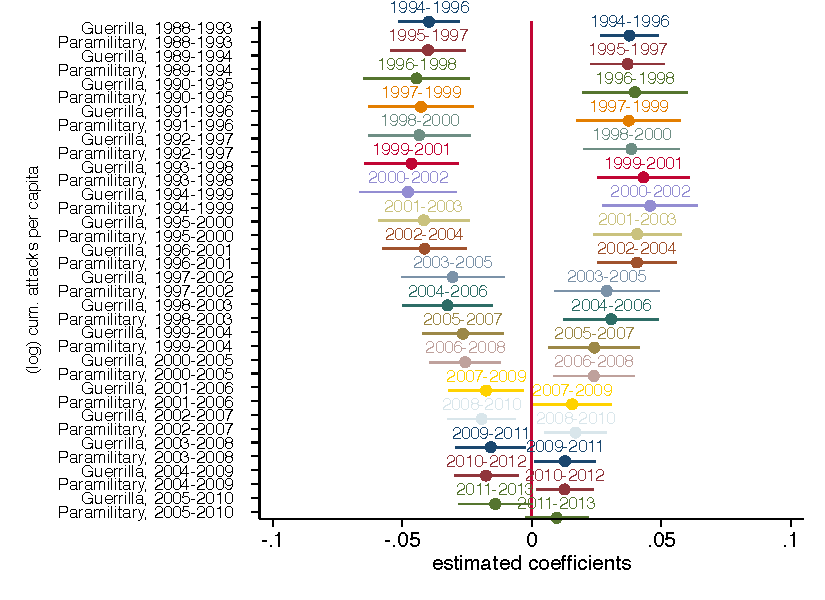
\includegraphics[width=1\textwidth]{Chapter3/Figures/figureE7.pdf}
\end{center}
\end{figure}

%--------------------------------
% FIGURE E2. EIGHT YEAR WINDOW
%--------------------------------

\begin{figure}[H]
\begin{center}
\caption{Estimated relationship between property tax revenues and attacks per armed group across Colombian municipalities, by time period using a moving window of 8 years}
\small{Dependent variable: (log) property tax revenue per capita (in the following 5-years)}
\label{appendix3:moving_window_8years}
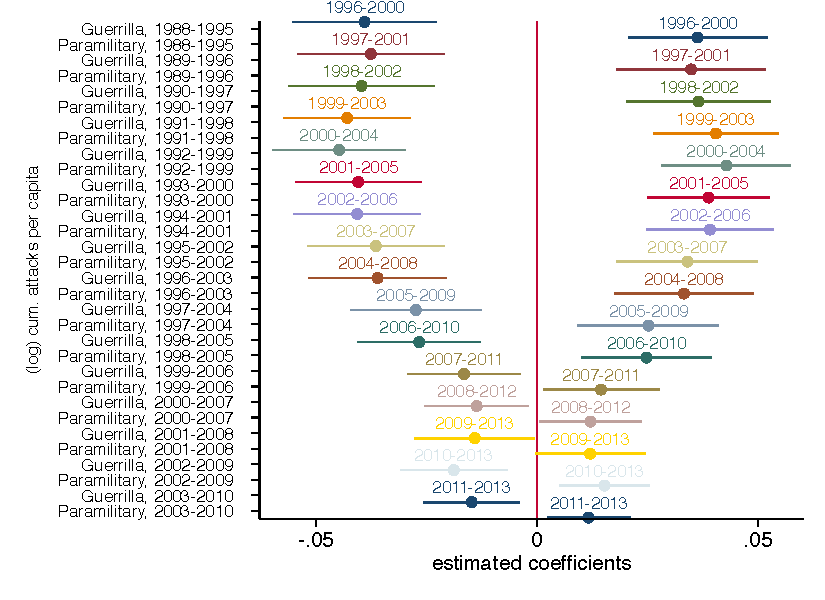
\includegraphics[width=1\textwidth]{Chapter3/Figures/figureE8.pdf}
\end{center}
\end{figure}

\newpage

%--------------------------------
\section{Multiple-testing correction \label{appendix3:multiple_test}}
%--------------------------------

The diversity of time periods, outcomes and mechanisms over the same dataset calls for the use of multiple-testing procedures to control for the familywise error rate (FWER), i.e. ``the probability of rejecting at least one true null hypothesis in a \emph{family} of tests'' (\citet{dafoeetal2017}). These procedures control for the inflation in false-positive error rates since there's a dependence across tests which increases the probability of getting a significant result by chance. Thus, we rely on three methods to deal with the multiple-testing problem: first, the Bonferroni correction -the most conservative approach- that adjusts the significance level $\alpha$ by setting the significance cut-off at $\alpha/n$, with $n$ the number of tests; second, the Hold correction, a less conservative approach to deal with the FWER, where after ordering the $j$ p-values from smallest to largest, selects the smallest one that would satisfy the condition $p_k > \alpha/(j+1-k)$, with $k$ the p-value's index, and from this level establishes a threshold at which smaller p-values are deemed as significant; lastly, the Benjamini-Hochberg procedure that controls for the False Discovery Rate (FDR), i.e. the expected proportion of false discoveries among all discoveries, where, after ordering the $j$th p-values, we find the largest one that satisfies the condition $p_k \leq (k/m)*\alpha$, and deems as significant all those lower than such threshold. 

Table \ref{appendix3:multiple_test_table} presents the correction results of the three procedures on the tests ran on Table \ref{chapter3_tab:main}, i.e. the relationships between cumulative attacks and tax revenues across four different time periods. The multiplication of time periods generates the aforementioned multiple-testing problem, thus pointing to the need for controlling for the FWER. After tacking into account the dependency across the 4 time periods, we note that even under the most conservative correction, i.e. Bonferroni, we still observe significant results for both treatment variables, and interestingly loose the significance in the last two periods where substantively we where not expecting results as is already noted in the main body of the paper (particularly in the last period). Note that under the Benjamini-Hochberg procedure, we still have significance for guerrilla attacks on the third period but not for paramilitaries, as expected. 

Furthermore, Table \ref{appendix3:multiple_test_table2} presents the correction comparisons and contrast to the target p-value $\alpha$ of 5\% for those tests that share the same treatment and outcome time period, 1997-2002 and 2003-2006, respectively. Given the diversity of mechanisms and outcomes over the same time period a concern is raised over the FWER. Correction results take into account all the outcomes of Tables \ref{chapter3_tab:main}, \ref{chapter3:table3}, \ref{chapter3:table4}, \ref{appendix3:consequences_violence} and \ref{appendix3:consequences_economic}, i.e. 11 tests. Results show that for the main outcome, property tax revenue per capita from Table \ref{chapter3_tab:main}, mechanisms of Table \ref{chapter3:table3}, and outcomes of Table \ref{appendix3:consequences_violence} (social outcomes), remain significant after the Bonferroni correction, and the number of significant tests increases when tacking into account either the Holm correction and the Benjamini-Hachberg procedure. No significant results are found for nighttime light data estimates (Table \ref{appendix3:consequences_economic}) either using 11 tests or 4 adjusting for 4 time periods, or for electoral outcomes after correction, except for the significance of the win dummy variable for Mayor election under the Benjamini-Hachberg procedure in column (9). 

\begin{table}[H]
\centering
\caption{Multiple-testing: corrections comparison and contrast to target p-value $\alpha$ of 5\% \\ \small{-Tests from Table \ref{chapter3_tab:main}-}}
\label{appendix3:multiple_test_table}
\scalebox{0.7}{
\begin{tabular}{lccccc}
 & \multicolumn{4}{c}{\textbf{Outcome}} &  \\ \cline{2-5}
DV: & \multicolumn{4}{c}{\textit{(log) property tax revenue per capita}} &  \\
DV time period: & 1997-2002 & 2003-2006 & 2007-2010 & 2011-20013 & \textbf{\begin{tabular}[c]{@{}c@{}}Statistically\\ \\ significant\end{tabular}} \\ \cline{2-5}
\textit{Benjamini-Hochberg procedure:} &  &  &  &  &  \\ \cline{1-1}
\begin{tabular}[c]{@{}l@{}}(log) cum. guerrilla attacks \\ per capita, over respective period\\ (1988-1996; 1997-2002;\\ 2003-2006; 2007-2010)\end{tabular} & \checkmark & \checkmark & \checkmark &  & 3/4 \\
\begin{tabular}[c]{@{}l@{}}(log) cum. paramilitary attacks \\ per capita, over respective period\\ (1988-1996; 1997-2002;\\ 2003-2006; 2007-2010)\end{tabular} & \checkmark & \checkmark &  &  & 2/4 \\
 &  &  &  &  &  \\
\textit{Holm correction:} &  &  &  &  &  \\ \cline{1-1}
\begin{tabular}[c]{@{}l@{}}(log) cum. guerrilla attacks \\ per capita, over respective period\\ (1988-1996; 1997-2002;\\ 2003-2006; 2007-2010)\end{tabular} & \checkmark & \checkmark &  &  & 2/4 \\
\begin{tabular}[c]{@{}l@{}}(log) cum. paramilitary attacks \\ per capita, over respective period\\ (1988-1996; 1997-2002;\\ 2003-2006; 2007-2010)\end{tabular} & \checkmark & \checkmark &  &  & 2/4 \\
 &  &  &  &  &  \\
\textit{Bonferroni correction:} &  &  &  &  &  \\ \cline{1-1}
\begin{tabular}[c]{@{}l@{}}(log) cum. guerrilla attacks \\ per capita, over respective period\\ (1988-1996; 1997-2002;\\ 2003-2006; 2007-2010)\end{tabular} & \checkmark & \checkmark &  &  & 2/4 \\
\begin{tabular}[c]{@{}l@{}}(log) cum. paramilitary attacks \\ per capita, over respective period\\ (1988-1996; 1997-2002;\\ 2003-2006; 2007-2010)\end{tabular} & \checkmark & \checkmark &  &  & 2/4 \\ \hline
\end{tabular}
}
\end{table}

\small{Note: This table presents multiple-testing corrections comparisons, and contrast to the target p-value of 5\%. It takes into account the 4 tests presented in Table \ref{chapter3_tab:main}. A \checkmark states a significant corrected estimate. Specifications used are the same as those found across Tables \ref{chapter3_tab:main}.} 

\begin{landscape}
\begin{table}[H]
\centering
\caption{Multiple-testing: corrections comparison and contrast to target p-value $\alpha$ of 5\% \\ \small{-Tests with treatment over period 1997-2002-}}
\label{appendix3:multiple_test_table2}
\scalebox{0.45}{
\begin{tabular}{lcccccccccccc}
 & \multicolumn{11}{c}{\textbf{Outcome}} &  \\ \cline{2-12}
\multicolumn{1}{c}{DV: time} & \multicolumn{11}{c}{\textit{2003-2006}} &  \\
\multicolumn{1}{c}{DV:} & \begin{tabular}[c]{@{}c@{}}Property\\  tax\\ revenue\end{tabular} & \begin{tabular}[c]{@{}c@{}}Per capita\\  land\\ value\end{tabular} & \begin{tabular}[c]{@{}c@{}}Cadastral\\  update\\ lag\end{tabular} & \begin{tabular}[c]{@{}c@{}}No. of\\  cadastral\\ updates\\  per capita\end{tabular} & \begin{tabular}[c]{@{}c@{}}Land \\ informality\\ rate\end{tabular} & \begin{tabular}[c]{@{}c@{}}Secondary \\ enrollmente\end{tabular} & \begin{tabular}[c]{@{}c@{}}Quality of\\  education\\ (math test)\end{tabular} & \begin{tabular}[c]{@{}c@{}}Nighttime\\  light\\ per capita\end{tabular} & \begin{tabular}[c]{@{}c@{}}Win\\ dummy,\\ Mayor \\ election\end{tabular} & \begin{tabular}[c]{@{}c@{}}Vote\\  share, \\ Mayor election\end{tabular} & \begin{tabular}[c]{@{}c@{}}Vote\\  share, \\ City \\ Council election\end{tabular} & \textbf{\begin{tabular}[c]{@{}c@{}}Statistically\\  significant\end{tabular}} \\ 
&(1) &(2)  &(3) &(4) &(5) &(6) &(7) &(8) &(9) &(10) &(11) \\
\cline{2-12}
\textit{Benjamini-Hochberg procedure:} &  &  &  &  &  &  &  &  &  &  &  &  \\ \cline{1-1}
\begin{tabular}[c]{@{}l@{}}(log) cum. guerrilla attacks \\ per capita, 1997-2002\end{tabular} & \checkmark & \checkmark & \checkmark & \checkmark & \checkmark & \checkmark & \checkmark &  & \checkmark &  &  & 8/11 \\
\begin{tabular}[c]{@{}l@{}}(log) cum. paramilitary attacks \\ per capita, 1997-2002:\end{tabular} & \checkmark & \checkmark & \checkmark & \checkmark & \checkmark & \checkmark & \checkmark &  & \checkmark &  &  & 8/11 \\
 &  &  &  &  &  &  &  &  &  &  &  &  \\
\textit{Holm correction:} &  &  &  &  &  &  &  &  &  &  &  &  \\ \cline{1-1}
\begin{tabular}[c]{@{}l@{}}(log) cum. guerrilla attacks \\ per capita, 1997-2002\end{tabular} & \checkmark & \checkmark & \checkmark & \checkmark & \checkmark & \checkmark & \checkmark &  &  &  &  & 7/11 \\
\begin{tabular}[c]{@{}l@{}}(log) cum. paramilitary attacks \\ per capita, 1997-2002:\end{tabular} & \checkmark & \checkmark & \checkmark & \checkmark & \checkmark & \checkmark & \checkmark &  &  &  &  & 7/11 \\
 &  &  &  &  &  &  &  &  &  &  &  &  \\
\textit{Bonferroni correction:} &  &  &  &  &  &  &  &  &  &  &  &  \\ \cline{1-1}
\begin{tabular}[c]{@{}l@{}}(log) cum. guerrilla attacks \\ per capita, 1997-2002\end{tabular} & \checkmark & \checkmark & \checkmark & \checkmark & \checkmark & \checkmark & \checkmark &  &  &  &  & 7/11 \\
\begin{tabular}[c]{@{}l@{}}(log) cum. paramilitary attacks\\ per capita, 1997-2002\end{tabular} & \checkmark & \checkmark & \checkmark & \checkmark & \checkmark &  & \checkmark &  &  &  &  & 6/11 \\ \hline
\end{tabular}

}
\end{table}
Note: This table presents multiple-testing corrections comparisons, and contrast to the target p-value of 5\%. It takes into account the 11 tests covered on the same time period, with the treatment variables running from 1997 to 2002, and outcome variables from 2003 to 2006. A \checkmark states a significant corrected estimate. Specifications used are the same as those found across Tables 2-4, \ref{appendix3:consequences_violence} and G2. 
\end{landscape}

\clearpage

\section{``Why This Matters'' \label{appendix3:why_matters}}

\subsection{Effect on social outcomes \label{appendix3:effect_social}}

Understanding the determinants of why some places are much better at collecting taxes than others is important for policy purposes. Municipalities in Colombia are responsible for providing a wide range of social goods that are likely to be affected by captured tax institutions. For instance, if tax revenues increase and they are invested in local social goods, then their quality should improve. In order to assess the effect of armed group presence on social outcomes, we evaluate educational outcomes for two reasons. First, educational outcomes  are very well measured at the municipal level in Colombia, and provide us a good way to gage the effect on social outcomes. On the other hand, their service might be more influenced by local dynamics relative to other public services that are dependent on national transfers and royalties. 

In this line, Table \ref{appendix3:consequences_violence} shows further that both guerrilla and paramilitary activity appear to have an asymmetric effect --consistent with the findings on tax revenues and tax institutions-- on educational attainment as well as education quality, as measured by the score in a standardized tests taken by all students finishing high school in the country (called SABER 11). Using the most demanding specification of column 2 of Table \ref{appendix3:consequences_violence}, an increase in cumulative per capita guerrilla attacks (paramilitary attacks) over the period 1997-2002 from the median to the 90$^{th}$ percentile of the distribution, is associated with an average drop (increase) of 19.6\% (17.2\%) of a standard deviation in the secondary enrollment rate over the period 2003-2006. The effect of a similar change on the quality of education as measured by the score in the math chapter of SABER 11 is a drop (increase) of 28\% (22\%) of a standard deviation for the case of cumulative guerrilla (paramilitary) attacks.

\subsection{Effect on economic activity \label{appendix3:effect_economic}}

To the best of our knowledge, no article has analyzed potential differential effects of guerrilla and paramilitary violence on economic activity.\footnote{\citet{riascosvargas2011} provide a thorough review the literature on the effect of armed conflict on economic performance in Colombia.}

In this appendix we investigate the effect of our cumulative conflict measure on local-level development, as measured by nighttime light  intensity, normalized by population. We find that cumulative violence perpetrated by guerrillas is consistently negatively associated with economic activity, while violence by paramilitaries is positively correlated, at least during the periods 2003-2006 and 2007-2010. 

Following the structure of Table \ref{chapter3_tab:main}, Table \ref{appendix3:consequences_economic} reports the estimates of the statistical association between guerrilla and paramilitary cumulative past violence and economic performance.

Odd columns show that the association between armed activity and economic performance is asymmetric across armed group: guerrilla cumulative attacks per capita have a negative relationship with economic activity (which is significant only in the second period) while paramilitary attacks show a positive
relationship (significant in all four periods). These results are, however, not robust to controlling for pre-period luminosity per capita (except in the third period for paramilitary attacks).

If we take into account the effect for the treatment period from 2003 - 2006 on 2007 - 2010 outcome, we notice a substantial asymmetric association. Because of the log-log specification, estimated coefficients should be interpreted as the elasticity of per capita property tax revenue with respect to cumulative past violence. 

Using the most demanding specification of column 6, an increase in cumulative per capita paramilitary attacks over the period 2003-2006 from the median to the 90$^{th}$ percentile of the distribution is associated with an average 3.5\% increase in nighttime lights over the period 2007-2010. 


\bigskip

% Table G1. Consequences: Cumulative violence (1997-2002) and social outcomes (2003-2006)

%\begin{landscape}
\begin{table}[htbp]
\def\sym#1{\ifmmode^{#1}\else\(^{#1}\)\fi}\caption{Consequences: Cumulative violence (1997-2002) and social outcomes (2003-2006)}
\label{appendix3:consequences_violence}
\begin{center}
\scalebox{0.65}{
\begin{tabular}{lccccc}
\hline \hline 
  & (1) & (2) & (3) & (4)   \\
 \hline 
 \\ 

 &\multicolumn{2}{c}{\emph{Secondary enrollment}}&\multicolumn{2}{c}{\emph{Quality of edu. (math test)}}\\\cmidrule(lr){2-3}\cmidrule(lr){4-5}
\addlinespace
\begin{tabular}[c]{@{}l@{}}Log guerrilla attacks\\ per capita \underline{1997-2002}\end{tabular}&     -0.0171\sym{***}&     -0.0088\sym{***}&     -0.0115\sym{***}&     -0.0092\sym{***}\\
            &    (0.0024)         &    (0.0021)         &    (0.0018)         &    (0.0018)         \\
\addlinespace
\begin{tabular}[c]{@{}l@{}}Log paramilitary attacks\\ per capita \underline{1997-2002}\end{tabular}&      0.0157\sym{***}&      0.0077\sym{***}&      0.0093\sym{***}&      0.0070\sym{**} \\
            &    (0.0024)         &    (0.0021)         &    (0.0019)         &    (0.0020)         \\
\addlinespace
Observations&        1071         &        1071         &         949         &         949         \\
R-squared   &       0.342         &       0.417         &       0.411         &       0.420         \\
Controls$^a$&  \checkmark         &  \checkmark         &  \checkmark         &  \checkmark         \\
Depto. FE   &  \checkmark         &  \checkmark         &  \checkmark         &  \checkmark         \\
Pre-period DV$^b$&                     &  \checkmark         &                     &  \checkmark         \\




\hline \hline 
\multicolumn{5}{p{1\textwidth}}{\footnotesize{Notes: Standard errors in parentheses are clustered at the department level; Significance-level: $^{***}$ 0.1\%; $^{**}$ 1\%; $^*$ 5\%; and $^{+}$ 10\%, refers to two-sided t-tests. 
$^a$Controls as in Table \ref{chapter3_tab:main}.
$^b$Due to the lack of quality of education data for the 1993-1996 period, we included the pre-period property tax revenue per capita from 1993 to 1996 in columns (2) and (4), to pick up part of the enduring cross-sectional within-department differences.}} \\
\end{tabular}
}
\end{center}
\end{table}
%\end{landscape}
%-----------------------------------------------------------%
\newpage

% Table G2. Consequences: Cumulative violence and economic activity

%\begin{landscape}
\begin{table}[htbp]
\def\sym#1{\ifmmode^{#1}\else\(^{#1}\)\fi}
\caption{Consequences: Cumulative violence and economic activity}
\label{appendix3:consequences_economic}
\begin{center}
\scalebox{0.65}{
\begin{tabular}{lcccccccc}
\hline \hline 
\multicolumn{9}{l}{Dependent variable: {\it Log of nighttime light per capita} over period:}\\

 &\multicolumn{2}{c}{1997-2002}              &\multicolumn{2}{c}{2003-2006}              &\multicolumn{2}{c}{2007-2010}              &\multicolumn{2}{c}{2011-2013}              \\\cmidrule(lr){2-3}\cmidrule(lr){4-5}\cmidrule(lr){6-7}\cmidrule(lr){8-9}
            &\multicolumn{1}{c}{(1)}         &\multicolumn{1}{c}{(2)}         &\multicolumn{1}{c}{(3)}         &\multicolumn{1}{c}{(4)}         &\multicolumn{1}{c}{(5)}         &\multicolumn{1}{c}{(6)}         &\multicolumn{1}{c}{(7)}         &\multicolumn{1}{c}{(8)}         \\
\addlinespace
\begin{tabular}[c]{@{}l@{}}Log guerrilla attacks\\ per capita \underline{1988-1996}\end{tabular}&     -0.0126         &      0.0008         &                     &                     &                     &                     &                     &                     \\
            &    (0.0125)         &    (0.0037)         &                     &                     &                     &                     &                     &                     \\
\addlinespace
\begin{tabular}[c]{@{}l@{}}Log paramilitary attacks\\ per capita \underline{1988-1996}\end{tabular}&      0.0314\sym{*}  &      0.0012         &                     &                     &                     &                     &                     &                     \\
            &    (0.0117)         &    (0.0032)         &                     &                     &                     &                     &                     &                     \\
\addlinespace
\begin{tabular}[c]{@{}l@{}}Log guerrilla attacks\\ per capita \underline{1997-2002}\end{tabular}&                     &                     &     -0.0269\sym{*}  &     -0.0003         &                     &                     &                     &                     \\
            &                     &                     &    (0.0103)         &    (0.0033)         &                     &                     &                     &                     \\
\addlinespace
\begin{tabular}[c]{@{}l@{}}Log paramilitary attacks\\ per capita \underline{1997-2002}\end{tabular}&                     &                     &      0.0458\sym{***}&      0.0016         &                     &                     &                     &                     \\
            &                     &                     &    (0.0098)         &    (0.0034)         &                     &                     &                     &                     \\
\addlinespace
\begin{tabular}[c]{@{}l@{}}Log guerrilla attacks\\ per capita \underline{2003-2006}\end{tabular}&                     &                     &                     &                     &     -0.0084         &     -0.0052         &                     &                     \\
            &                     &                     &                     &                     &    (0.0099)         &    (0.0031)         &                     &                     \\
\addlinespace
\begin{tabular}[c]{@{}l@{}}Log paramilitary attacks\\ per capita \underline{2003-2006}\end{tabular}&                     &                     &                     &                     &      0.0364\sym{***}&      0.0070\sym{*}  &                     &                     \\
            &                     &                     &                     &                     &    (0.0086)         &    (0.0030)         &                     &                     \\
\addlinespace
\begin{tabular}[c]{@{}l@{}}Log guerrilla attacks\\ per capita \underline{2007-2010}\end{tabular}&                     &                     &                     &                     &                     &                     &     -0.0193         &      0.0144         \\
            &                     &                     &                     &                     &                     &                     &    (0.0220)         &    (0.0090)         \\
\addlinespace
\begin{tabular}[c]{@{}l@{}}Log paramilitary attacks\\ per capita \underline{2007-2010}\end{tabular}&                     &                     &                     &                     &                     &                     &      0.0469\sym{*}  &     -0.0069         \\
            &                     &                     &                     &                     &                     &                     &    (0.0195)         &    (0.0079)         \\
\addlinespace
Observations&        1028         &        1028         &        1045         &        1045         &        1048         &        1048         &        1048         &        1048         \\
R-squared   &       0.547         &       0.920         &       0.600         &       0.953         &       0.660         &       0.975         &       0.665         &       0.963         \\
Controls$^a$&  \checkmark         &  \checkmark         &  \checkmark         &  \checkmark         &  \checkmark         &  \checkmark         &  \checkmark         &  \checkmark         \\
Depto. FE   &  \checkmark         &  \checkmark         &  \checkmark         &  \checkmark         &  \checkmark         &  \checkmark         &  \checkmark         &  \checkmark         \\
Pre-period DV$^b$&                     &  \checkmark         &                     &  \checkmark         &                     &  \checkmark         &                     &  \checkmark         \\


\hline \hline
\multicolumn{9}{p{1.4\textwidth}}{\footnotesize{Notes: Standard errors in parentheses are clustered at the department level; Significance-level: $^{***}$ 0.1\%; $^{**}$ 1\%; $^*$ 5\%; and $^{+}$ 10\%, refers to two-sided t-tests. 
$^a$ Controls as in Table \ref{chapter3_tab:main}.
$^b$ Estimations include pre-period logged luminosity per capita from 1992 in column (2), from 1992 to 1996 in (4), from 2000 to 2002 in (6), and from 2003 to 2006 in (8), to pick up part of the enduring cross-sectional within-department differences.}} \\
\end{tabular}
}
\end{center}
\end{table}
%\end{landscape}

\clearpage


\section{Civil war dynamics and capture in Colombia: the four periods in more detail} \label{fourperiods}

The dynamics of the civil war in terms of territorial control and violence have changed significantly over time.\footnote{Differences also exist within the groups across regions, we summarize the broad trends.}

We separate the war's recent evolution, and the armed groups' capture strategies, into four periods. We organize the statistical analysis around these four periods because pooling them would effectively assume that armed actors had the same ability to influence tax policies in every year, which strikes us as substantively unrealistic. Importantly, levels of violence and control by different groups varied across these periods, a fact that we exploit in our empirical strategy.

\textbf{1988-1996: FARC ascendancy}\\
The FARC increased its presence in the mid-1980s and 1990s. According to one estimate \citep[28]{echandia06a}, in 1985, the FARC had a presence in 173 of the country's roughly 1,120 municipalities, and by 1995 spread to 622. During this period, the FARC tried to influence policy directly by forming a political party, the Patriotic Union (UP), that began to contest local elections in 1988.  UP candidates won sixteen mayoral positions and 256 municipal council positions. Only two years later, though, the UP distanced itself from the FARC to protect itself from the violence targeted at them by paramilitary groups. By the end of the period, the FARC and the ELN both enforced election boycotts in areas under their control, and threatened elected mayors and local council members \citep{el-tiempo97a}. 

While some regional politicians supported paramilitaries' formation during this period \citep[37]{ronderos14a}, e.g. Pablo Emilio Guar\'{i}n from the Liberal party, there is little evidence that paramilitary groups tried to capture political institutions directly at the local level. This is not to say that there were no political impacts of paramilitary presence during this period. In areas experiencing paramilitary violence, like the Magdalena Medio and Urab\'{a}, high levels of displacement and political assassination were endemic. These processes surely affected the viability of some candidates and forms of politics during this period.  

\textbf{1997-2002: Paramilitary expansion}\\
In 1997, regional paramilitary groups united under the umbrella group United Self-Defense Forces of Colombia (AUC) and the war spread. By 2001, the AUC was powerful enough to convene a meeting with nearly 100 politicians to formulate a concerted effort to win elections at all levels, and to support \'Alvaro Uribe's candidacy for president in 2002 (known as the Santa Fe de Ralito pact). According to the attorney general's office, the Sante Fe de Ralito pact was an effort by the paramilitaries to use their ``consolidated'' military and economic power at the local levels ``to influence the Congress as a political actor and prepare for an eventual negotiation process'' \citep{verdad-abierta15a}. 

The details of how this effort played out are informative about how military power was transformed into political influence.\footnote{Vicente Casta\~{n}o, one of the brothers behind the formation of the AUC, apparently ordered AUC blocks to enter politics, with the idea that the groups would be recognized as political organizations rather than drug traffickers, and be eligible for more lenient criminal charges as a result \citep{ronderos14a}.} 
One commander in Urab\'{a} excelled at political organizing: Fredy Rend\'{o}n Herrera, alias `El Alem\'{a}n' (The German), and head of the Elmer C\'{a}rdenas block (ECB). The block entered the northern region of Urab\'{a} and accompanied the army's ``Operation Genesis,'' which involved the mass displacement of many communities and the eventual takeover by the paramilitaries. In 2000, El Alem\'{a}n began to train wounded combatants as ``Social Development Promoters'' to organize communities under their control, and specifically to form JACs and carry out projects together, such as road and bridge building \citep{verdad-abierta15b}. The JACs were then used as the basis for electoral influence: ahead of the 2001 elections, they convened assemblies within communities to choose candidates for the municipal councils. For mayor, El Alem\'{a}n reported in his confession to authorities that the strategy was to select two candidates: one with similar ideological preferences as the AUC, and one that had little political clout, so could easily be controlled. By 2010, 25 politicians from the region were convicted of collaboration with the paramilitaries. The block also engaged in electoral coercion, according to \citet{avila-martinez10a}.\footnote{The paramilitaries also formed a political alliance with municipal governments in the region called ``For a Big, United Urab\'{a} at Peace.'' VerdadAbierta.com, an investigative journalism organization, reported that the Elmer C\'{a}rdenas block used its political connections to ``take advantage of the productive projects [related to coca eradication] as well as the public finances of the municipalities under its control.'' The block even evaluated projects presented to the municipal council, or proposed its own projects, according to one ex-combatant's testimony. In 2002, the block also formed a non-profit organization called ASOCOMUN, which competed and won municipal contracts and grants from the central government \citep{verdad-abierta15b}. Finally, by 2002, the AUC decided to support particular candidates for Congress, in order to try to influence a favorable demobilization agreement with the government. All candidates backed by El Alem\'{a}n in Urab\'{a} were elected \citep{verdad-abierta11a}.} 

Compared to the paramilitaries, the FARC's influence remained indirect. The FARC largely continued to eschew official electoral politics during this period, preferring to target municipal candidates that the group did not approve of, or acting mayors. This targeting presumably created strong incentives for local politicians in areas of dominant FARC presence to shift their policies towards the group's preferences. A key exception is the territory it governed directly during peace talks with the Pastrana administration (1998-2002). Known as the \emph{Zona de Despeje}, the territory included 6 municipalities and was roughly the size of Maryland. During this period, the FARC enacted \emph{Ley 002} to govern taxation, which stipulated who would be taxed (the wealthy), and the consequences for not paying (kidnapping) \citep{farcley2005}. The first article of the law established the tax collection for those individuals or companies with assets worth more than a million dollars, without specifying the rate, while the second article stated that failing to pay the stated tax would imply an increase of the tax amount (again without stating the tax value and rate). Finally, according to the third article of the law, those that didn't comply would be detained until a suitable payment would be made (\citet{farcley2005}). . In 2002, the Pastrana administration ended peace talks and reentered the Maryland-sized zone comprising six municipalities it had ceded to the FARC during the talks, known as the. FARC tax policy in the \emph{despeje} provides evidence of its preferences for informality and favoritism of the poor and landless.
This was an extension of the FARC's early practice of taxing the local population in areas where it established its earliest presence \citep{molano87a}. 

\textbf{2003-2006: Paramilitary demobilization} \\
In 2003, the Uribe administration negotiated a ceasefire with paramilitary groups and eventually adopted the {\it Justice and Peace law}. The law allowed paramilitary commanders to demobilize their troops in exchange for lenient sentences, with a maximum of eight years total possible prison time.\footnote{Uribe also extradited 14 commanders to the US in 2008 for failing to comply with the condition of confessing all of their crimes; they are now serving longer prison sentences for drug trafficking convictions.} 
Paramilitary demobilizations began in 2003 and reached a peak in 2005, which officially transformed the war into a contest between the state and remaining insurgent groups (the FARC and ELN). In total, by 2006, 37 paramilitary blocks had demobilized \citep{altocomisionado06}. 

In spite of the demobilization program, some groups remained active and continued to exert an influence on local politics. For example, the ECB continued to influence local politics through 2006, including ``check-ins'' with the mayors' secretaries \citep{verdad-abierta11a}. According to one former paramilitary commander's confession, the point was not to control the mayoral offices, but to ``help them deliver development to the people'' \citep{verdad-abierta11a}.  

The conflict with the FARC continued apace during this period, but there was no clear change in terms of capture strategy. In Urab\'{a}, for example, El Alem\'{a}n's block continued to deepen its influence in local politics, and also turned their attention to the national level, through pacts with regional political elites \citep{gutierrez-sanin10c, lopez-hernandez10a}. They formed groups of candidates who would rotate in office, one year at a time \citep{verdad-abierta11a}. Interestingly, none of the three candidates for Congressional representative backed by the Elmer C\'{a}rdenas block won election for the 2006-2010 period (candidates for Senate, elected at large, however, did receive unusually high vote shares in the region). At the local level, ASOCOMUN continued to win grants and contracts, amounting to what VerdadAbierta.com calculated was \$1.607 million pesos (roughly \$500k).

\textbf{2007-2010: State resurgence}\\
Besides the remaining left-wing guerrilla groups, many former paramilitary groups morphed into new organizations, including the ``Black Eagles,'' and drug-trafficking groups such as the ``Urabe\~{n}os'' and the ``Rastrojos.'' All of these groups sometimes engaged in actions against the FARC, the ELN, and the civilian population. \footnote{See \citet{daly16a} for an account of the variation in post-demobilization trajectories and the emergence of criminal bands (BACRIMs).} Some have also attacked leaders of groups seeking land restitution, presumably to block efforts to invalidate titles that were acquired through coercion or violence \citep{amnesty-international14a}. 

Under Uribe, the Colombian military and police redeployed to major population centers and roads, improving measures of security. In addition, government forces killed several members of the FARC's secretariat, including Alfonso Cano, who had taken over the leadership of the group following Manuel Marulanda's death in 2008. The weakened FARC agreed to peace talks following the 2010 election of Uribe's Minister of Defense, Juan Manuel Santos. 




